\documentclass[12pt,twoside]{report}

\author{
  Oliver Kohlbacher, Heiko Klein,\\
  Andreas Kerzmann, Andreas Moll, Andreas K\"{a}mper
}
\title{
  \begin{center}
    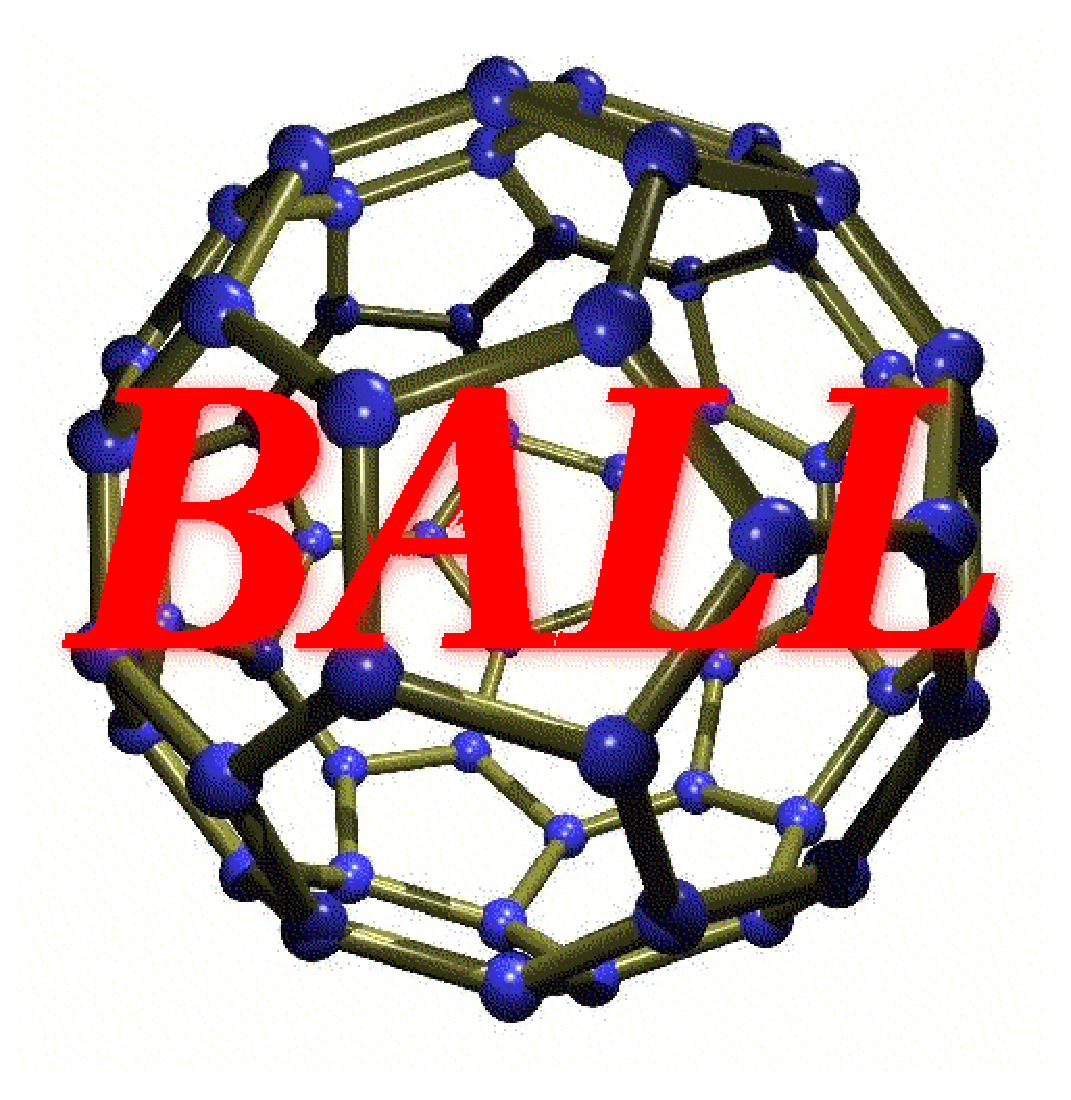
\includegraphics[width=9cm]{logo.eps}
  \end{center}
  \Huge BALL\\ 
  \Large A Tutorial
}
\date{
  Release 1.2\\
  \today
}

\usepackage{longtable}
%-----------------------------------------
% used packages
%-----------------------------------------
\usepackage{a4}
% use A4 paper

%\usepackage[draft]{graphicx}
\usepackage{graphicx}
% use graphics pacakge

\usepackage{times}
% use postscript fonts

\usepackage{psboxit}
\newcommand{\graybox}[1]{\psboxit{box .85 setgray fill}{\fbox{#1}}}
% display gray shaded boxes using postscript commands
%


%-----------------------------------------
% quote environment for quatations
%-----------------------------------------
% in part stolen from LaTeX companion
\usepackage{ifthen}
\newsavebox{\QuoteNameBox}
\newenvironment{Quote}[1]%
	{%
		\sbox{\QuoteNameBox}{{\it #1}}%
		\begin{list}{}{%
			\setlength{\rightmargin}{\leftmargin}}%
				\item[]``\ignorespaces}%
	{\unskip''\hfill \usebox{\QuoteNameBox}\end{list}}


\usepackage{changebar}
% This package defines the two commands \cbstart and \cbend. It then displays a
% bar between the start and the end command

\usepackage{color}
% This package allows the coloring of text (e.g. in an ipe minipage)

\usepackage{float}
% the float package allows a better placement of all floats (figures,tables) or
% even new floats it allows the following kinds of boxes:
% \shadowbox, \doublebox, \ovalbox, \Ovalbox

\makeatletter
	\renewcommand{\@makecaption}[2]{
		\vspace{3pt}
		\noindent{\color{blue}\rule{\textwidth}{1pt}}\par
		\noindent{\small{\sffamily #1:}\hspace{5pt}\itshape #2\par}
		\vspace{5pt}
	}
\makeatother
% 
%  create a fancy float caption: 
%    - blue rule under the float
%    - the figure text set in sans serif
%    - the caption text in italics

\setcounter{topnumber}{1}
\setcounter{bottomnumber}{1}
%
%  	some settings for the floats: just on float at the
%		top of a page and on at the bottom

	
%-----------------------------------------
% Font definitions 
%-----------------------------------------

\usepackage{amsfonts}
\usepackage{amsmath}
\usepackage{amsthm}
\usepackage{amssymb}

%-----------------------------------------
% Textlayout 
%-----------------------------------------

\newcommand{\clearemptydoublepage}{\newpage{\pagestyle{empty}\cleardoublepage}}

%\usepackage{a4wide}
\setlength{\textheight}{21cm}
\setlength{\textwidth}{14.5cm}
\setlength{\oddsidemargin}{10mm}
\setlength{\evensidemargin}{2mm}
\setlength{\topmargin}{0mm}
%\setlength{\marginparsep}{5mm}
%\setlength{\marginparwidth}{2cm}
%\renewcommand{\baselinestretch}{1.21}
\large\normalsize

%-----------------------------------------
% some shorthands
%-----------------------------------------

\providecommand{\R}{\mathbb R}
\providecommand{\Q}{\mathbb Q}
\providecommand{\N}{\mathbb N}
\providecommand{\Z}{\mathbb Z}

%-----------------------------------------
% redefinitions of sectioning comands
%-----------------------------------------

\usepackage{fancyheadings}
% allows you an easy adaption of the headings

\usepackage{fancybox}
% you can use shaded boxes e.g. for figures it allows the following kinds of boxes:
% \shadowbox, \doublebox, \ovalbox, \Ovalbox

\addtolength{\headrulewidth}{0.2pt}
\addtolength{\footrulewidth}{0.6pt}
\addtolength{\headwidth}{1cm}
\addtolength{\footskip}{10mm}
\addtolength{\headsep}{5mm}
\addtocounter{secnumdepth}{2}
\setcounter{tocdepth}{3}
\setcounter{secnumdepth}{3}

\renewcommand{\chaptermark}[1]{\hfill\markboth{#1}{}\hfill}
\renewcommand{\sectionmark}[1]{\hfill\markright{\thesection\ #1}\hfill}
\lhead{}
\rhead{}
\chead[\fancyplain{}{\textrm{\leftmark}}]%
      {\fancyplain{}{\textrm{\rightmark}}}
\cfoot{}
\rfoot[\fancyplain{}{}]{\fancyplain{}{\bfseries\thepage}}
\lfoot[\fancyplain{}{\bfseries\thepage}]{\fancyplain{}{}}


% the \chapter ...
\makeatletter
%\renewcommand\thesection 			{{\sffamily\thechapter.\@arabic\c@section}}
%\renewcommand\thesubsection   {{\sffamily\thesection.\@arabic\c@subsection}}
%\renewcommand\thesubsubsection{{\sffamily\thesubsection.\@arabic\c@subsubsection}}
\renewcommand{\@chapapp}{\sffamily}
%\renewcommand\section{\@startsection {section}{1}{\z@}%
%	{-3.5ex \@plus -1ex \@minus -.2ex}%
%	{2.3ex\@plus.2ex}%
%	{\normalfont\Large\sffamily\bfseries}
%}
%\renewcommand\subsection{\@startsection{subsection}{2}{\z@}%
%	{-3.25ex\@plus-1ex \@minus -.2ex}%
%	{1.5ex \@plus .2ex}%
%	{\normalfont\large\sffamily\bfseries}
%}
%\renewcommand\subsubsection{\@startsection{subsubsection}{3}{\z@}%
%	{-3.25ex\@plus-1ex \@minus -.2ex}%
%	{1.5ex \@plus .2ex}%
%	{\normalfont\normalsize\sffamily\bfseries}
%}
\makeatother

%-----------------------------------------
% macro for missing pieces
%-----------------------------------------
\usepackage{changebar}
\newcommand{\missing}[1]{
	\cbstart  % add a gray bar at the side of the page
	\message{^^JMISSING: #1^^J}
	\par\noindent\fbox{{\bf MISSING:} #1}\par
	\cbend
}

%-----------------------------------------
% rules for figures
%-----------------------------------------

\topfigrule
\botfigrule
\setlength{\shadowsize}{2pt}

%-----------------------------------------
% some shorthands
%-----------------------------------------

\usepackage{xspace}
% you should use \xspace in defining shorthands 
% e.g. \newcommand{\eg}{e.g., \xspace} \@ is for the correct spacing after punctuation

\newcommand{\eg}{{\it e.g.}\xspace}
\newcommand{\ie}{{\it i.e.}\xspace}
\newcommand{\ea}{{\it et al.}\xspace}
\newcommand{\etc}{{\it etc.}\xspace}
\def\CPP{C\raise.08ex\hbox{\tt ++}\xspace}


%-----------------------------------------
% the index
%-----------------------------------------
\usepackage{makeidx}

\newcommand{\Index}[1]{#1\index{#1}}
% prints the term and creates an index entry

\newcommand{\class}[1]{{\ttfamily{#1}}\index{#1@{\ttfamily{#1}}
(BALL~class)}\index{BALL!classes!#1@{\ttfamily{#1}}}}
% BALL class names are typeset in typewriter bold and indexed automatically:
%  - first with their class name
%  - then under BALL!classes!<classname>

\newcommand{\STLclass}[1]{{\ttfamily{#1}}\index{#1@{\ttfamily{#1}}
(STL~class)}\index{STL!#1 class@{\ttfamily{#1}}}}
% STL class names are typeset in typewriter bold and indexed automatically:
%  - first with their class name
%  - then under STL!<classname> class

\newcommand{\function}[1]{{\ttfamily{#1}}\index{#1@{\ttfamily{#1}}
(BALL~function)}\index{BALL!functions!#1@{\ttfamily{#1}}}}
% BALL function names are typeset in typewriter bold and indexed automatically:
%  - first with their name
%  - then under BALL!functions!<function name>

\newcommand{\method}[1]{{\ttfamily{#1}}\index{#1@{\ttfamily{#1}}
(method)}\index{BALL!functions!#1@{\ttfamily{#1}}}}
% method names are typeset in typewriter bold and indexed automatically:
%  - first with their name
%  - then under BALL!methods!<function name>

\newcommand{\attribute}[2]{{\ttfamily{#1}}\index{#1@{\ttfamily{#2}}
({\ttfamily #1} attribute)}\index{BALL!!#1!#2@{\ttfamily{#1}}}}
% attribute names are typeset in typewriter bold and indexed automatically:
%  - first with their name and (<class> attribute)
%  - then under BALL!<class>!<attribute>

\newcommand{\macro}[1]{{\ttfamily{#1}}\index{#1@{\ttfamily{#1}}
(BALL~macro)}\index{BALL!macros!#1@{\ttfamily{#1}}}}
% BALL macros names are typeset in typewriter bold and indexed automatically:
%  - first with their name
%  - then under BALL!macros!<macro name>

\newcommand{\namespace}[1]{{\ttfamily{#1}}\index{#1@{\ttfamily{#1}}
(BALL~namespace)}\index{BALL!namespaces!#1@{\ttfamily{#1}}}}
% BALL macros names are typeset in typewriter bold and indexed automatically:
%  - first with their name
%  - then under BALL!namespaces!<name>

\newcommand{\type}[1]{{\ttfamily{#1}}\index{#1@{\ttfamily{#1}}
(BALL~type)}\index{BALL!types!#1@{\ttfamily{#1}}}}
% BALL macros names are typeset in typewriter bold and indexed automatically:
%  - first with their name
%  - then under BALL!types!<macro name>

\newcommand{\file}[1]{
	{\ttfamily\mbox{#1}}
	\index{#1@{\ttfamily{#1}} (file)}
}
% BALL file names are typeset in typewriter bold and indexed automatically:
% with their name and "(file)" appended

\newcommand{\directory}[1]{
	{\ttfamily\mbox{#1}}
	\index{#1@{\ttfamily{#1}} (directory)}
}
% BALL directories are typeset in typewriter bold and indexed automatically:
% with their name and "(directory)" appended

\newcommand{\option}[1]{
	{\ttfamily\mbox{#1}}
	\index{configure!options!#1@{\ttfamily\mbox{#1}}}
}
% BALL file names are typeset in typewriter bold and indexed automatically:
% as configure/options/<name>"

\newcommand{\exception}[1]{{\ttfamily{#1}}\index{#1@{\ttfamily{#1}}
(BALL~class)}\index{BALL!exceptions!#1@{\ttfamily{#1}}}}
% BALL exceptions names are typeset in typewriter bold and indexed automatically:
%  - first with their name
%  - then under BALL!exceptions!<exception name>

\newcommand{\newtermdef}[1]{{\em #1}\index{#1!definition}}
% prints the term in italics and includes creates an index entry
% with the subentry "definition"

\newcommand{\newterm}[1]{{\em #1}\index{#1}}
% prints the term in italics and creates an index entry

\newcommand{\URL}[1]{{\bfseries\ttfamily\mbox{#1}}}
\newcommand{\email}[1]{{\bfseries\ttfamily\mbox{#1}}}

%--------------------------------------------
%  the style of embedded listings
%--------------------------------------------
\usepackage{listings}
% formatting of the listings
\lstset{
	%% we use ANSI C++
	language=[ANSI]C++,
%
	%% our tabs are always expanded to 2 blanks
	tabsize=2,
%
	%% the font size of the listing
	basicstyle=\small\ttfamily,
%
	%% make the listing as wide as \textwidth
	spread=-0.3cm,
%
	%% draw a line at the left of the listing
	frame=tlrb,
%
	%% captions appear at the bottom of the listing
	%captionpos=b,
%
	%% and make the corners of the frame round
	frameround=tttt,
%
	%% the label font
	labelstyle=\sffamily,
%
	%% line numbers for each line
	labelstep=0
}
\newcommand{\linelisting}{\lstinline[frame=,basicstyle=\small]}


%%
%%
%%     FAQ macros
%%
\newcounter{FAQcounter}
\setcounter{FAQcounter}{0}
\newcommand{\FAQquestion}[1]{%
	\ifthenelse{\theFAQcounter=0}{}{\vspace{0.5cm}\begin{center}\rule{0.5\textwidth}{1pt}\end{center}\vspace{0.5cm}}%
	\stepcounter{FAQcounter}%
	\noindent{\bf Question \theFAQcounter:} {\em #1 \par}%
}
\newcommand{\FAQanswer}[1]{\bigskip\noindent{\bf Answer:} #1\par}	
\newcommand{\FAQURL}[1]{{\tt #1}}

\pagestyle{fancyplain}
\sloppy
\makeindex

\begin{document}
\setlength{\headheight}{14.5pt}
\pagenumbering{roman}
\setcounter{page}{1}
\maketitle
\cleardoublepage

% \pagestyle{fancyplain}
\tableofcontents
\clearpage

\pagenumbering{arabic}
\setcounter{page}{1}


\chapter{Introduction}
\label{chapter:introduction}
\noindent
BALL (Biochemical Algorithms Library) is an application framework for rapid
software prototyping in the field of Molecular Modeling.  This tutorial shall
help new users to make their first steps with BALL. It is {\em not} a full
documentation. For a full documentation, please refer to the \newterm{Reference
Manual}~\cite{BALL-RM} which can be obtained in HTML, PDF, or postscript format.

There are also several papers and technical reports published on
BALL~\cite{BKL99a,BKL99b,KL99,Koh2001,KL2000,MHLK05,MHLK06}
that give a cursory overview of its design principles and illustrate its use in
Rapid Software Prototyping. If you publish results that were obtained using 
BALL, please cite it as follows:
\begin{enumerate}
  \item[] O. Kohlbacher, H.-P. Lenhof: BALL -- Rapid Software Prototyping
          in Computational Molecular Biology, {\em Bioinformatics} 2000,
          16(9):815--824
\end{enumerate}

\noindent
The latest version of BALL, bug fixes, and updates are available from our 
website

\begin{enumerate}
  \item[] \URL{http://www.ball-project.org}
\end{enumerate}

\noindent 
as well as further documentation, bug reports, and changes.

The next section of this tutorial gives a short overview of the structure and
contents of BALL. Chapter \ref{chapter:getting-started} describes the
installation and related issues. In Chapter \ref{chapter:first-steps}, some
fundamental concepts and classes are explained. After that we will show how to
use more advanced features of BALL. We will have a general overview of BALL 
 (Chapters \ref{chapter:foundation-classes} and  \ref{chapter:kernel}) 
and the usage of the visualization parts of BALL (Chapter \ref{chapter:view-programming}). 
Chapter \ref{chapter:python} will show you
the mechanisms and the usage of BALL's Python bindings.  Finally, Chapter
\ref{chapter:faq} tries to answer some of the most frequently asked questions.

\section{Overview}
\index{BALL!overview}

The basis of all BALL classes is an extensive set of \newterm{foundation
classes}.  They provide generic implementations of advanced data structures
(\eg, trees, hash associative containers, hash grids, \etc), mathematical
objects (\eg, matrices, vectors, geometric objects), implementations of
\Index{design patterns}, object \Index{persistence}, and access to the
operating system (\eg, networking support, file handling). An overview of the
overall structure of BALL is given in Fig. \ref{fig:BALL_structure}.

The BALL \newterm{kernel} contains the molecular data structures for the
representation of atoms, bonds, molecules, proteins, \etc  The kernel classes
are implemented with the foundation classes and are carefully designed to
provide maximum extensibility and flexibility.
\begin{figure}[tb]
  \centering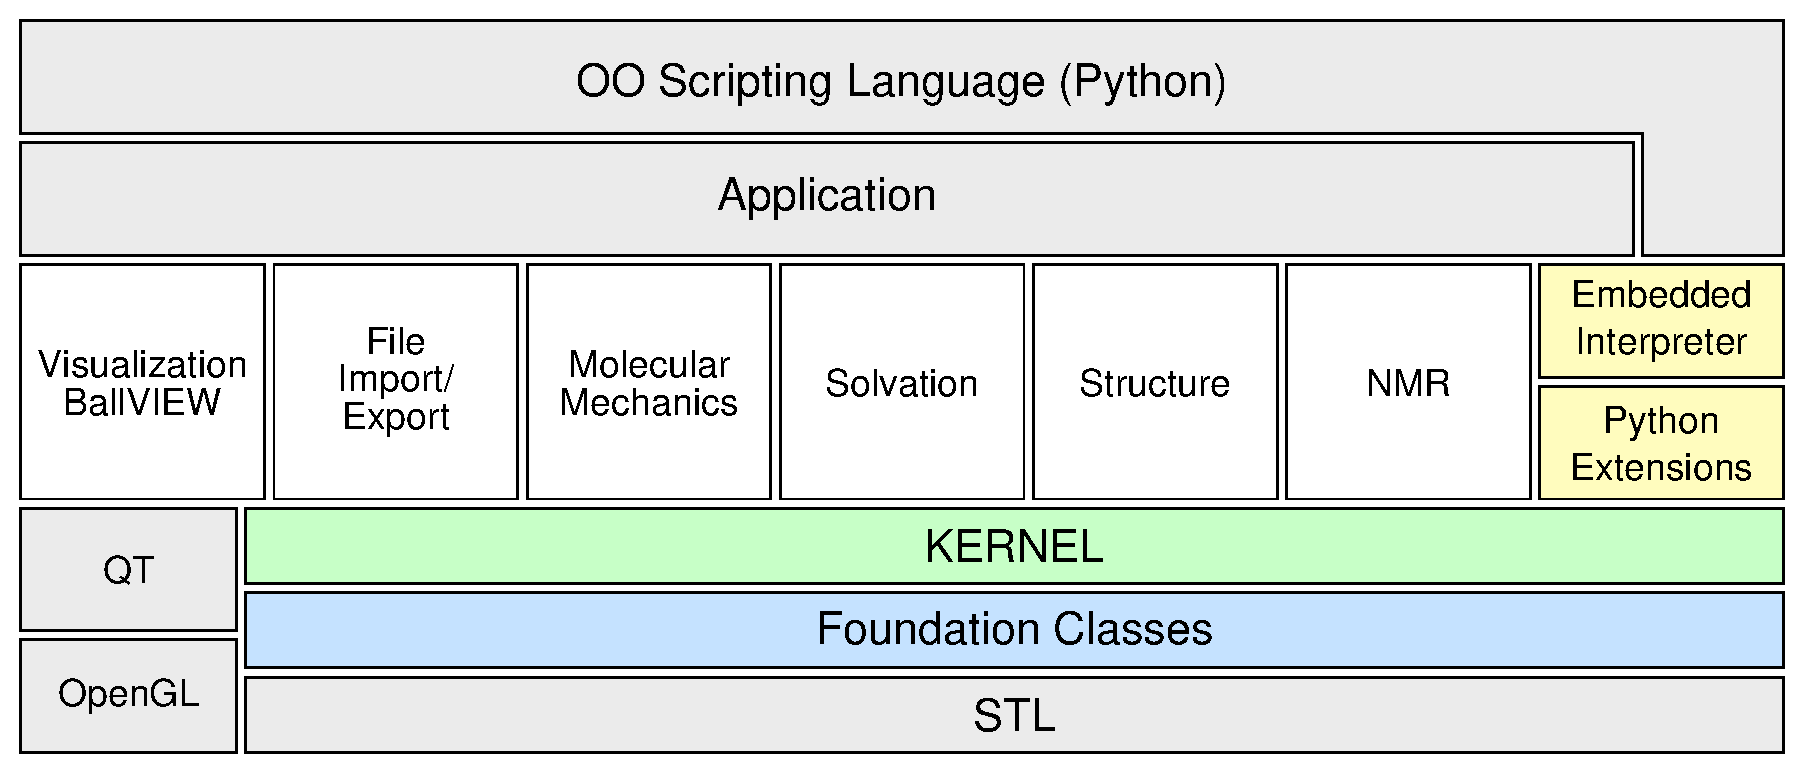
\includegraphics[width=\textwidth]{BALL_structure.eps}
  \caption{Overview of the structure of BALL}
  \label{fig:BALL_structure}
\end{figure}

The third layer of classes (on top of the foundation classes and the kernel)
provides the functionality required for applications. We call them
\newterm{basic components}. Each of these basic components is independent of
the other components.  We have implemented five basic components that cover
\Index{Molecular Mechanics}, file import/export, advanced \Index{solvation
methods}, structure analysis/comparison and \Index{visualization}. These
areas were selected, because our main interest stems from the field of protein
docking. The Molecular Mechanics component does not only provide standard
force fields (AMBER~\cite{AMBER95}, CHARMM~\cite{BBO+83}), but also a generic
\Index{force field}.  This generic force field is a base class for all force
fields. It implements fundamental methods to manage parameter files, parameter
assignment, and atom type assignment, and defines a common interface for all
force fields. Thus, large portions of code may be reused for the
implementation of new force fields.  The file import/export component
implements general methods for efficient file handling, but also methods to
read and write the most common file formats used for molecular structures
(\eg, PDB, MOL2). The solvation component provides methods for calculating
solvation effects. The first method that accounts for solvation is the atomic
contact energy by Zhang {\it et al.}~\cite{ZVC+97}. The second approach that
we implemented is a numerical solver for the \Index{Poisson-Boltzmann} equation.  The
structure component contains algorithms to search for common structural motifs
in proteins, to map molecules onto each other, and to calculate solvent
accessible and solvent excluded surfaces of molecules. For the visualization
of the results, we designed \Index{VIEW}, a class hierarchy that
visualizes BALL kernel objects with standard representations (ball and stick,
van der Waals, ribbons, surfaces, \etc). The visualization was implemented
using OpenGL and QT~\cite{QT}. Hence, it is highly portable and enables the
user to produce state-of-the-art graphical user interfaces with a minimum
effort.

The fourth layer in BALL consistes of Python bindings. Python is an
object-oriented scripting language that is easy to learn and very readable.
BALL provides Python bindings for most of its classes, which allow the use of
the BALL \CPP classes from Python. This approach drastically reduces the
turn-around times (no compiling and linking phase is required) and adds
scripting capabilities to BALL without introducing a new and exotic scripting
language. The Python bindings use the same class names as the BALL classes,
therefore after the initial rapid development of a methodology, the existing
Python code can be easily ported back to \CPP for production purposes.
Chapter \ref{chapter:python} gives a short introduction to this feature.



\chapter{Getting Started}
\label{chapter:getting-started}
\section{System Requirements}

\subsection{Compiler}
\index{compiler}
  BALL requires a (more or less) ANSI compliant \CPP compiler.
  It has been successfully built and tested on the following platforms:
	\begin{itemize}	
   	\item Linux/x86 2.x using g{\tt ++} 3.2.1
   	\item Linux/x86 2.x using g{\tt ++} 2.95.3
%   	\item Linux/x86 2.x using Kuck \& Associate (KAI) \CPP 4.0
%   	\item Linux/x86 2.x using Intel Compiler 5.0
   	\item Solaris/SPARC 8 using g{\tt ++} 3.2.1
   	\item Solaris/SPARC 8 using g{\tt ++} 2.95.3
%   	\item Solaris/SPARC 8 using Kuck \& Associate (KAI) \CPP 4.0
   	\item Solaris/SPARC 8 using Sun Forte Developer 7 C++ 5.4 2002/03/09
   	\item IRIX 6.5 using CC 7.3.1.1m (32 and 64 bit)
%   	\item Compaq Tru64 Unix V4.0f using Compaq \CPP 6.3
		\item Microsoft Windows XP using Microsoft Visual Studio .NET (MSVC 7.0)
 	\end{itemize}

\subsection{External software and libraries}
BALL needs {\tt flex} and {\tt bison} for automatically generating parsers
for various purposes. These utilities are standard software and should be
installed on every contemporary UN*X machine. The newest versions are
downloadable from \URL{http://www.gnu.org/software/}.

The usage of GNU make is recommended, although BALL will also build with
other versions of make. It is available from \URL{ftp://ftp.gnu.org/gnu/}
and easy to install.

The compilation of the visualization component BALLVIEW also requires
the QT library (version 3.0.6) which is available from
\URL{http://www.troll.no/qt}/.

If QT was not installed in one of the standard library paths or the
QT header files were not installed in one of the compiler's default
include directories, use \mbox{"\option{--with-qt-libs}{\tt{}=DIR}"} and
\mbox{"\option{--with-qt-incl}{\tt{}=DIR}"} as options to configure (see
Section \ref{section:building-ball}) to specify the paths QT was installed
to.\index{QT}
Please remember to compile also \file{libqgl.so}, which is one of the QT
extensions (to build \file{libqgl.a}, cd to 
{\tt\nobreak{\$QTDIR/extensions/opengl/src}} and type {\tt make}).

QT also requires OpenGL. On platforms that do not provide OpenGL, MESA can
be used (e.g. Linux). Mesa is a 3-D graphics library with an API which is 
very similar to that of OpenGL. It can be obtained from 
\URL{http://www.mesa3d.org}.
\index{MESA}

To use the Python extensions of BALL (Python is an object oriented
scripting language), you will also need Python 2.1 installed
(\URL{http://www.python.org}) and a special version of SIP 3.0 distributed
through our website (\URL{http://www.mpi-sb.mpg.de/BALL/}). SIP is a tool
for generating Python bindings for C++ class libraries.

Additionally you need might need the FFTW package for fast Fourier
transformations (Verson 2.1.3), available from \URL{http://www.fftw.org/}.

Please make sure that the required external \CPP libraries (i.e. QT and SIP)
have been compiled with the same compiler (and compiler version!) as the BALL
libraries. Otherwise you will most likely see a plethora of strange error
messages, either while linking applications or at runtime.

\section{Installation}
\label{section:building-ball}

Building BALL is very easy, but please read through this section carefully to
avoid any problems.  If all requirements stated above are met, BALL is built
by issuing the following commands in the directory {\tt BALL/source}:

\begin{lstlisting}{}
  ./configure
  make
\end{lstlisting}

The following sections give further details on the configuration of the library,
on the library files created, how to test the library, and how to build BALL 
applications.

\subsection{Configuring BALL}
\index{configure!usage}

"{\tt configure}" tries to gather as much information on your system as possible and 
then creates the necessary configuration files (\file{config.h},
\file{config.mak}, \file{common.mak}, and \file{Makefile}).
The configuration of BALL may be adapted to your needs and to your system
configuration from the command line by adding one or more of the options from
Table \ref{table:options}.
An overview of these options can also be obtained by executing "{\tt configure
--help}"

% \begin{center}
\begin{longtable}{lp{7cm}}\hline
  \option{--x-includes}{\tt{}=DIR}&        X include files are in DIR\\\vspace{3mm}

  \option{--x-libraries}{\tt{}=DIR}&       X library files are in DIR\\\vspace{3mm}

  \option{--enable-optimization}&          optimize the library for speed, remove debug info\\\vspace{3mm}

  \option{--enable-debuginfo}&             create debug information\\\vspace{3mm}

  \option{--disable-BALLVIEW}&             disable the compilation of BALLVIEW, the visualization
                                           component\\\vspace{3mm}

  \option{--enable-64}&                    build 64 bit objects (if allowed
                                           by the compiler)\\\vspace{3mm}

  \option{--with-compiler}{\tt{}=CXX}& use CXX to compile BALL\\\vspace{3mm}

  \option{--with-cxxflags}{\tt{}=FLAGS}&   add FLAGS to the \CPP compiler flags
                                           (commas are converted to blanks)
                                           \\\vspace{3mm}

  \option{--with-ldflags}{\tt{}=FLAGS}&    add FLAGS to the linker flags
                                           (commas are converted to blanks)
                                           \\\vspace{3mm}

  \option{--with-arflags}{\tt{}=FLAGS}&    add FLAGS to the flags for the
                                           creation of the static libraries
                                           \\\vspace{3mm}

  \option{--with-dynarflags}{\tt{}=FLAGS}& add FLAGS to the flags for the
                                           creation of the shared libraries
                                           \\\vspace{3mm}

  \option{--with-qt-incl}{\tt{}=DIR}&      QT header files are in DIR\\
                                           \vspace{3mm}

  \option{--with-qt-libs}{\tt{}=DIR}&      QT libraries are in DIR\\\vspace{3mm}
	\option{--with-moc}{\tt{}=MOC}& 					The absolute path to the QT meta object
																						compiler (moc, typically found in
																						{\tt\$QTDIR/bin/moc})\\\vspace{3mm}

	\option{--with-threadsafe-qt}& 						Set this flag if you the multi-threaded
																						version of Mesa and you compiled
																						the thread-safe version of QT\\\vspace{3mm}
			
  \option{--with-opengl-incl}{\tt{}=DIR}&  OpenGL/Mesa header files are in DIR/GL\\\vspace{3mm}

  \option{--with-opengl-libs}{\tt{}=DIR}&  OpenGL/Mesa libraries are in DIR/GL\\\vspace{3mm}

  \option{--with-mesa}&                    use MESA instead of OpenGL\\
                                           \vspace{3mm}

  \option{--without-libxnet}&              use \Index{libsocket}/\Index{libnsl}
                                           for linking rather than 
                                           \Index{libxnet} (under Solaris)
                                           \\\vspace{3mm}

  \option{--with-python=EXE}& 							Enable Python support using the
																						Python executable in EXE.
Typically, from the executable {\tt configure} can figure out where the
headers and the library are hidden, so that the following two options are
usually not required.\\\vspace{3mm}
  
  \option{--with-python-incl=DIR}&         Python includes (Python.h) is in
                                           DIR\\\vspace{3mm}

  \option{--with-python-libs=DIR}&         Python library (libpython*.a) is
                                           in DIR\\\vspace{3mm}

  \option{--with-python-ldopts=X}&         Use additional options X when
                                           linking with the Python library
                                           \\\vspace{3mm}

  \option{--with-sip-lib=DIR}&             the SIP library resides in DIR
                                           \\\vspace{3mm}

  \option{--with-sip-incl=DIR}&            the SIP header file resides in DIR
                                           \\\vspace{3mm}

  \option{--with-sip=DIR}&                 the SIP executable resides in DIR
                                           \\\vspace{3mm}

  \option{--without-xdr}&                  no RPC/XDR headers available - do
                                           not build portable binary
                                           persistence support
                                           \\\vspace{3mm}

  \option{--help}&                         display help information\\\hline
\caption{options for {\tt configure}}
\label{table:options}
\end{longtable}
%\end{center}
%\caption{options for {\tt configure}}
%\label{table:options}

For example, to compile BALL without the visualization component BALLVIEW,
specify 
\begin{lstlisting}{}
  configure --disable-BALLVIEW
\end{lstlisting}

To include BALLVIEW using the QT installation in /opt/qt/lib and /opt/qt/include, specify

\begin{lstlisting}{}
  configure --with-qt-libs=/opt/qt/lib 
		--with-qt-incl=/opt/qt/include
\end{lstlisting}

If Mesa should be used (when compiling under Linux), the correct options might look
like this:

\begin{lstlisting}{}	
  configure --with-qt-libs=/opt/qt/lib 
		--with-qt-incl=/opt/qt/include
    --with-opengl-libs=/opt/mesa/lib 
		--with-opengl-incl=/opt/mesa/include
\end{lstlisting}

\subsection{Building the Libraries}

After the successful termination of configure, issuing "make" will build the
shared libraries. Three different libraries will be built:
\begin{center}
	\begin{tabular}{ll}
  	\file{libBALL.so}&     the main BALL library\\
  	\file{libVIEW.so}&     the visualization component BALLVIEW\\
	  \file{libMOLVIEW.so}&  the molecule--related part of BALLVIEW\\
	\end{tabular}
\end{center}

The latter two libraries are not built if "\option{--disable-BALLVIEW}" is specified or configure
cannot find X libraries, OpenGL libraries, or QT libraries (and the respective headers).

It is also possible (although not recommended) to build the corresponding static libraries
\file{libBALL.a}, \file{libVIEW.a}, and \file{libMOLVIEW.a} using "{\tt make
staticlibs}". Please note that statically linked binaries are huge.

\subsection{Installing the Libraries}

After compiling the libraries, they are installed in {\tt BALL/lib/\${BINFMT}/}
when calling "{\tt make install}" where {\tt \${BINFMT}} is the binary format
as determined by {\tt configure}.  Currently, the only way to install the
libraries somewhere else is by moving them by hand to the desired destination.
Wherever you install the shared libraries, please make sure to include their
location in the \Index{{\tt LD\_LIBRARY\_PATH}} environment variable.

If you are using \Index{csh}, \Index{tcsh}, or similar shells, use the command
\begin{lstlisting}{}
   setenv LD_LIBRARY_PATH DIR
\end{lstlisting}

\noindent to set the library path. If you are using \Index{sh}, \Index{bash},
or related shells, try

\begin{lstlisting}{}   
   LD_LIBRARY_PATH=DIR
   export LD_LIBRARY_PATH
\end{lstlisting}

If you installed the shared libraries in a directory that the dynamic linker
\Index{ld} searches by default, it is not necessary to set {\tt
LD\_LIBRARY\_PATH}.

\section{Testing the Library}
\index{testing}
\index{test programs}

\subsection{Unit Tests}

BALL provides an extensive suite of test programs to ensure the correctness of
the code on all platforms. This test suite requires a lot of patience since
the compilation takes quite some time. However, we recommend to run these
tests to ensure that the library is fully operational. The test programs are
located in the directory {\tt BALL/source/TEST}. To compile and run the test
suite, use "{\tt make test}". Please make sure that {\tt LD\_LIBRARY\_PATH} is
correctly set, otherwise the execution of the test programs will fail.

Each of the test programs tests one or more classes of BALL. When a test
program (\eg~{\tt Atom\_test}) is run, the program prints either "OK" (if all
tests passed) or "FAILED" if any of the tests failed. "{\tt make test}" runs
all tests and complains if a certain test fails.  


If this happens, please let report a bug through our online bug tracking
system at \URL{http://ball-trac.bioinf.uni-sb.de}.

\noindent
For all bug reports, please include your system configuration, the file
\file{config.log} (which contains the results of tests configure performed),
and the file \file{BALL/include/BALL/config.h} (which contains the compiler
defines used by BALL).

\subsection{Benchmarks}

If you want to know how fast the version of BALL is compared to other systems,
you might want to run the benchmark suite in \directory{BALL/source/BENCHMARKS}.
You can compile the benchmark suite by changing to that directory and running
"{\tt make}". After that, run the benchmarks with "{\tt make bench}".
Depending on your hardware and whether you compiled BALL with or without
optimization, running the benchmarks will take up to several minutes. Upon
termination, it will print an overall number, the BALLStones. This number is a
crude estimate of the performance you can expect for a mix of typical BALL
applications. The benchmark suite currently includes benchmarks for the BALL
kernel data structures, file I/O, the AMBER force field, and the
Poisson-Boltzmann solver. The BALL web site contains a list of benchmark
results for different platforms, please feel free to submit your results for
inclusion.

\include{building-python}

\chapter{First Steps With BALL}
\label{chapter:first-steps}
\section{Building molecules}

Since BALL is intended for Molecular Modeling, the classes representing atoms,
bonds, and molecules are of central importance. In this first example, we will
construct a water molecule ``by hand'' to illustrate the use of these classes.
Typical applications would read molecular structures from a file. This will be
shown in the second example.

\noindent
To start the construction of a water molecule, we first create an (empty)
\Index{atom}. Atoms are represented by the class \class{Atom}.

\begin{lstlisting}{}
	Atom* oxygen = new Atom;
\end{lstlisting}
	
\noindent
Atoms have a number of attributes. As we created this atom without specifying
any of its properties, these attributes are set to their defaults. The
following table lists the attributes of an atom along with its
\newtermdef{accessors} (methods to access or modify an attribute) and default
values.
\begin{center}
	\begin{tabular}{lllc}
	attribute		&	type				& accessors     						& default\\
	\hline
	name				& String			& setName,getName						& {\tt ""}\\
	element			& Element			& setElement,getElement			& {\tt Element::UNKNOWN}\\
	charge			& float				& setCharge,getCharge				& 0.0\\
	radius			& float				& setRadius,getRadius				& 0.0\\
	type name   & String			& setTypeName,getTypeName		& {\tt ""}\\
	type        & Atom::Type	& setType,getType						& {\tt Atom::INVALID\_TYPE}\\
	position    & Vector3			& setPosition,getPosition		& (0, 0, 0)\\
	velocity    & Vector3			& setVelocity,getVelocity		& (0, 0, 0)\\
	force		    & Vector3			& setForce,getForce					& (0, 0, 0)
	\end{tabular}
\end{center}

\noindent
For example, we can assign the \Index{element} for our new atom:

\begin{lstlisting}{}
	oxygen->setElement(PTE[Element::O]);
\end{lstlisting}

\noindent
The expression {\tt PTE[\class{Element}::O]} returns an instance of class
\class{Element}. It is assigned to our atom using the \method{setElement}
method. We leave our new atom at the default position (0, 0, 0) and create two
new atoms, which will be the still missing hydrogen atoms:

\begin{lstlisting}{}
	Atom* hydrogen1 = new Atom;
	Atom* hydrogen2 = new Atom;
	hydrogen1->setElement(PTE[Element::H]);
	hydrogen2->setElement(PTE[Element::H]);
\end{lstlisting}
	
\noindent
Now we have to assign the correct coordinates to the two hydrogen atoms.  The
method \method{setPosition} takes an instance of \class{Vector3} as an
argument. This class is used to represent coordinates and vectors in
three--dimensional space. An object of type \class{Vector3} can be constructed
from three floating point numbers which represent the x, y, and z coordinates.
Thus, we can assign the coordinates as follows:
 
\begin{lstlisting}{}
 	hydrogen1->setPosition(Vector3(-0.95, 0.00, 0.0));
 	hydrogen2->setPosition(Vector3( 0.25, 0.87, 0.0));
\end{lstlisting}

\noindent

Now, our three atoms are of the right type and at the right positions. However, we
do not yet have a molecule, so let's create one:\\

\begin{lstlisting}{}
	Molecule* water = new Molecule;
\end{lstlisting}

\noindent
Molecules are representd by the \class{Molecule} class. Each instance of this
class may contain an arbitrary number of atoms. Using the \method{insert}
method, we can construct a molecule from our atoms:

\begin{lstlisting}{}
	water->insert(*oxygen);
	water->insert(*hydrogen1);
	water->insert(*hydrogen2);
\end{lstlisting}

\noindent
For a complete water molecule, we still need two \Index{bonds}. This can be
achieved with the method \method{createBond}:
	
\begin{lstlisting}{}
	oxygen->createBond(*hydrogen1);
	oxygen->createBond(*hydrogen2);
\end{lstlisting}

or

\begin{lstlisting}{}
	hydrogen2->createBond(*oxygen);
\end{lstlisting}

\noindent
To verify that everything worked as expected, we might print the number of
atoms in the molecule or the number of bonds for each atom:
	
\begin{lstlisting}{}
	cout << "# of atoms in water: " 
 			 << water->countAtoms() << endl;
	cout << "# of bonds of oxygen: " 
			 << oxygen->countBonds() << endl;
	cout << "# of bonds of hydrogen1: " 
		   << hydrogen1->countBonds() << endl;
	cout << "# of bonds of hydrogen2: " 
			 << hydrogen2->countBonds() << endl;
\end{lstlisting}

\noindent
The method \method{countAtoms} is available for all kernel classes that might
contain atoms and returns the total number of atoms for this object. The
method \method{countBonds} returns the number of bonds the atom shares. An
atom can have at most eight bonds.

We can also verify the bond distances:
\begin{lstlisting}{}
	Vector3 bond_vector = oxygen->getPosition() 
										    - hydrogen1->getPosition();

	cout << "bond distance: " 
			 << bond_vector.getLength() << endl;
\end{lstlisting}
	
\noindent
\method{getPosition} is the complementary method of \method{setPosition}: it
returns the current position of an atom. The return value is again of type
\class{Vector3}. The length of this vector is then returned by the
\method{getLength} method. 

Water molecules rarely occur alone, so we are going to create further water.
All BALL kernel classes are container classes and support \newterm{deep
copying}, \ie when assigned or copy constructed their contents are copied as
well. So, we can easily create a new water molecule:

\begin{lstlisting}{}
	Molecule* water2 = new Molecule(*water);
\end{lstlisting}
	
\noindent
This molecule is an exact copy of our original water molecule. Especially, the
atoms have the same position as in the original. So we want to shift the whole
molecule to another position.  In principle, we could access all atoms in the
copy and add a constant translation vector to their position. However, there
is a simpler way. BALL provides so--called \newterm{processors}. These
processors may be applied to any of the kernel objects and perform an
operation on any objects they encounter. For example the
\class{TranslationProcessor} performs a simple translation on every atom it
finds. The use of the processors is very simple.  All kernel classes define an
\method{apply} method wich takes a processor as an argument. In order to
translate our second water molecule by a certain distance, we first create a
\class{TranslationProcessor}:

\begin{lstlisting}{}
	TranslationProcessor translation(Vector3(5, 0, 0));
\end{lstlisting}
	
\noindent
The translation vector is specified as the argument of the constructor. Now we
may translate the atoms of our water molecule by a simple call to \method{apply}

\begin{lstlisting}{}
	water2->apply(translation);
\end{lstlisting}

\noindent
Another important kernel class besides atoms and molecules is \class{System}.
A system is a collection of atoms, molecules, or any other kernel objects. For
example, we can store our two water molecules in a system object:

\begin{lstlisting}{}
	System S;
	S.insert(*water);
	S.insert(*water2);
\end{lstlisting}

\begin{figure}[t]
	\centering
	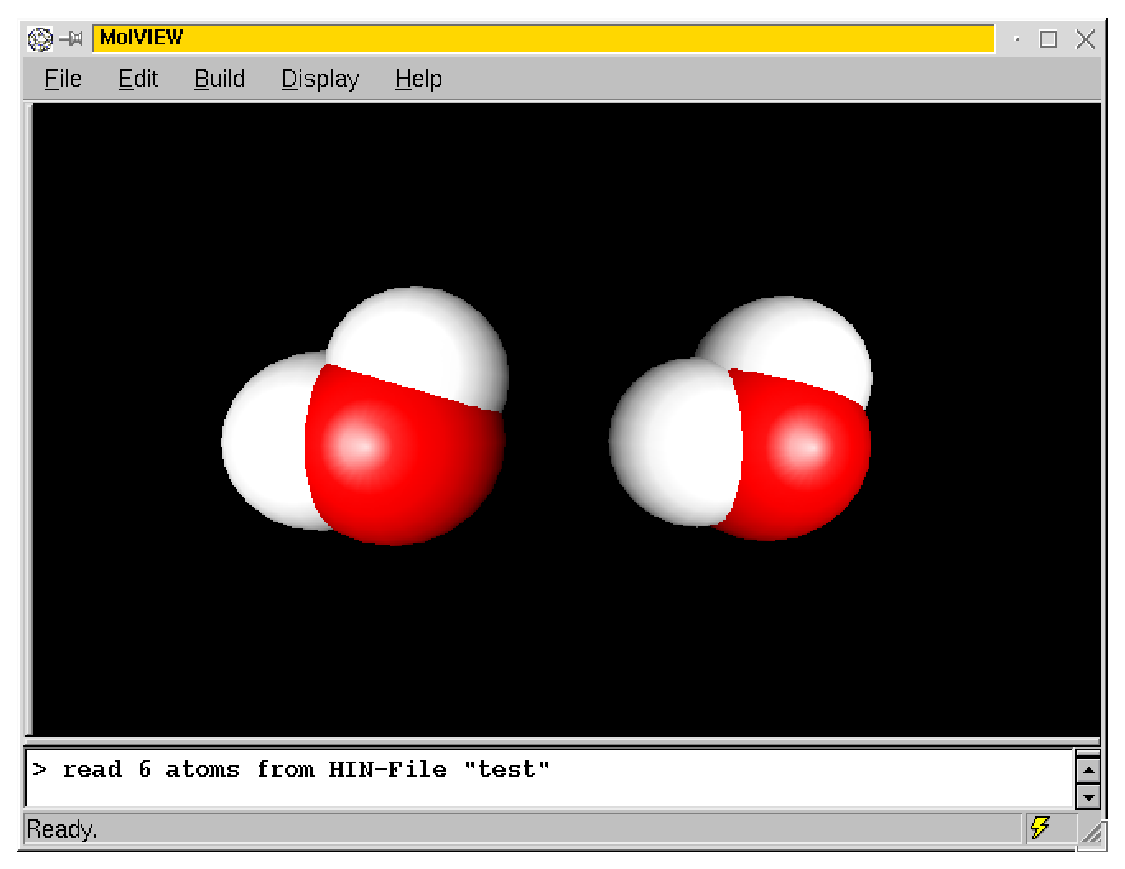
\includegraphics[width=\textwidth]{tut1_screenshot}
	\caption{Screenshot of BALLView showing the result of the first example
					 ({\tt tutorial1.C})}
	\label{fig:tut1-screenshot}
\end{figure}
\noindent
We can now manipulate the two water molecules simultaneously. For example a
further application of the translation processor to the system would apply
the translation to both molecules.
But now we would like to have a look at what we built. So we might write our
system to a file and inspect it with a molecule viewer (\eg BALLView).
BALL supports a variety of file formats. For example we could write the system
to a HyperChem HIN file~\cite{HyperChem}:
\begin{lstlisting}{}
	HINFile outfile("water.hin", File::OUT);
	outfile << S;
	outfile.close();
\end{lstlisting}
\noindent
These three lines of code create a \class{HINFile} object which is used to
read and write HyperChem files. The first line opens a file named {\tt
water.hin} for output ({\tt File::OUT}; if the second argument is omitted the
file is opened for reading only).
The second line uses the stream operator {\tt <<} to write the contents
of system {\tt S} to this file. The file is closed in the third line.

% ????? [anker]
% The following is not true. If we use a pointer here, then it's OK, but
% with a System it simply doesn't work. What do we want here? I'd prefer a
% Sytsem instead of a System*.

% Finally, we have to delete all the objects we created. This is very simple:
% 
% \begin{lstlisting}{}
% 	delete S;
% \end{lstlisting}

\noindent 
As all molecules and atoms we created are inside the system, they are deleted
automatically as soon as the system is deleted.

If this short program is run it creates the following output:

\begin{lstlisting}[frameround=]{}
	# of atoms in water: 3
	# of bonds of oxygen: 2
	# of bonds of hydrogen1: 1
	# of bonds of hydrogen2: 1
	bond distance: 0.95
\end{lstlisting}

\noindent
It also creates a file named {\tt water.hin} which contains the two water
molecules. Fig.~\ref{fig:tut1-screenshot} shows the contents of this file
in the BALLView viewer.

To compile this small example, we still have to include a few header files.
The complete file is shown in Listing~\ref{lst:tutorial1} on
page~\pageref{lst:tutorial1} and can be found in \mbox{{\tt
BALL/source/TUTORIAL/tutorial1.C}}.

First, we have to include \file{iostream} as we use {\tt cout} and {\tt endl}
to print some text. Then, we have to include the headers for the BALL kernel
classes \class{Atom}, \class{Bond}, \class{Molecule}, \class{System}, and
\class{PTE}. The headers for the HyperChem file support are found in the
directory \directory{BALL/FORMAT} and the headers for the
\class{TranslationProcessor} class are found in
{\tt BALL/STRUCTURE/geometricProperties.h}.

As all BALL classes are hidden in the \namespace{BALL} namespace, we have to
give access to this namespace with the command 
\begin{lstlisting}{}
	using namespace BALL;
\end{lstlisting}
Similarly, we also use the namespace \namespace{std} which contains {\tt cout}
and {\tt endl}.

If you have BALL installed, you might now try to compile this example. Simply
change to the directory \directory{BALL/source/TUTORIAL} which contains all
the examples from this tutorial and type 
\begin{lstlisting}[frameround=]{}
	make tutorial1
	./tutorial
\end{lstlisting}
This should build and execute the example. Please remember to set the
environment variable {\tt LD\_LIBRARY\_PATH} to the directory where your
libraries are installed.

After the successful execution of the example, a file named {\tt water.hin}
should appear in the current directory. This file contains the two water
molecules. You might inspect it with the molecule viewer BALLView.
Fig.~\ref{fig:tut1-screenshot} shows a screenshot of BALLView displaying the two
water molecules.

\newpage
\begin{lstlisting}[captionpos=t,caption={The complete source code of the first example.}\label{lst:tutorial1}]{}
// tutorial example 1
// ------------------
// build two water molecules and write them to a file

// needed for cout
#include <iostream>

// the BALL kernel classes
#include <BALL/KERNEL/atom.h>
#include <BALL/KERNEL/bond.h>
#include <BALL/KERNEL/molecule.h>
#include <BALL/KERNEL/system.h>
#include <BALL/KERNEL/PTE.h>

// reading and writing of HyperChem files
#include <BALL/FORMAT/HINFile.h>

// the TranslationProcessor
#include <BALL/STRUCTURE/geometricTransformations.h>

// we use the BALL namespace and the std namespace
using namespace BALL;
using namespace std;

int main()
{
	// we create a new atom called oxygen
	// and set its element to oxygen (PTE[Element::O])
	Atom* oxygen = new Atom;
	oxygen->setElement(PTE[Element::O]);

	// now we create two hydrogen atoms...
	Atom* hydrogen1 = new Atom;
	Atom* hydrogen2 = new Atom;
	hydrogen1->setElement(PTE[Element::H]);
	hydrogen2->setElement(PTE[Element::H]);

	// ...and move them to approximately correct positions
 	hydrogen1->setPosition(Vector3(-0.95, 0.00, 0.0));
 	hydrogen2->setPosition(Vector3( 0.25, 0.87, 0.0));

	// We create our water molecule...
	Molecule* water = new Molecule;

	// ...and insert the three atoms into the molecule.
	water->insert(*oxygen);
	water->insert(*hydrogen1);
	water->insert(*hydrogen2);

	// Then we build the two O-H bonds
	oxygen->createBond(*hydrogen1);
	oxygen->createBond(*hydrogen2);

	// Some statistics: Molecule::countAtoms() 
	// returns the number of atoms, Atom::countBonds() 
	// the number of bonds the atom shares
	cout << "# of atoms in water: " 
			 << water->countAtoms() << endl;
	cout << "# of bonds in oxygen: " 
			 << oxygen->countBonds() << endl;
	cout << "# of bonds of hydrogen1: " 
			 << hydrogen1->countBonds() << endl;
	cout << "# of bonds of hydrogen2: " 
			 << hydrogen2->countBonds() << endl;

	// bond_vector is a vector and is set to the
	// difference of atom positions of oxygen and hydrogen1
	Vector3 bond_vector = oxygen->getPosition() 
											- hydrogen1->getPosition();

	// Vector3::getLength: the length of the vector
	cout << "bond distance: " 
			 << bond_vector.getLength() << endl;

	// Now we copy our molecule using a copy constructor.
	Molecule* water2 = new Molecule(*water);

	// A translation processor moves the second molecule
	// 5 Angstrom along the x axis
	TranslationProcessor translation(Vector3(5, 0, 0));
	water2->apply(translation);

	// We insert our two molecules into a system
	System* S = new System;
	S->insert(*water);
	S->insert(*water2);

	// and write this system to a HyperChem file
	HINFile outfile("water.hin", File::OUT);
	outfile << *S;
	outfile.close();

	// We delete the system. This also deletes 
	// the molecules and the atoms therein
	delete S;
}
\end{lstlisting}

\section{Handling proteins}

In the second example we take a step towards real world applications. Instead
of constructing our own molecules, we now read a protein from a \newterm{PDB
file}. The PDB format~\cite{PDB} is a standardized file format for molecular structure
data. In our case, we will read BPTI (bovine pancreatic trypsin inhibitor), a
small protein:

\begin{lstlisting}{}
	PDBFile infile("bpti.pdb");
	System S;
	infile >> S;
	infile.close();
\end{lstlisting}

\noindent
In the first line, we create a \class{PDBFile} object and assign it to a file
named {\tt bpti.pdb}. Then we create an empty system {\tt S} and read the
contents of the PDB file into the system using the stream operator {\tt >>}.
This use of the stream operators is possible for all file formats in BALL (see
also the first example). Hence, you can easily switch file formats
by changing just the type of the {\tt infile} object (\eg replace it by
\class{HINFile} to read HyperChem files).

We can now verify whether the file was correctly read. BPTI should have 594
atoms. As said before, the number of atoms in any kernel object that might
contain atoms (\ie all classes that are derived from \class{AtomContainer}) is
obtained by calling \method{countAtoms}:

\begin{lstlisting}{}
	cout << "# of atoms in BPTI: " << S.countAtoms() << endl;
\end{lstlisting}

Now, we are interested in the sequence of BPTI. Since BPTI contains only a
single chain, we might just traverse all residues of this chain and write
their names to {\tt cout}. This is done by \newterm{iterators}. Iterators are
objects that can be used to traverse container objects (\eg lists, arrays, or
-- in our case -- proteins). Iterators ``point'' to an element of a container
object. They may be incremented to get the next element and they may be
derferenced similar to pointers by using {\tt *} or {\tt ->}. In fact,
C pointers can be thought of as iterators.
The use of iterators in BALL is similar to the
use of iterators in the \newterm{Standard Template Library} (\Index{STL}).
But there is a significant difference. STL containers usually contain objects of
one single type (\eg a list of strings). In BALL kernel objects, this is
different. A system may contain atoms, proteins, molecules, residues, \etc
This leads to a difference in the interface. A typical {\tt for} loop using STL
iterators to access all elements of a list looks as follows:

\begin{lstlisting}{}
	list<string> string_list = ...;
	list<string>::iterator list_it;
	
	for (list_it = string_list.begin(); 
			 list_it != string_list.end();
			 ++list_it)
	{
		cout << *list_it << endl;
	}
\end{lstlisting}

\noindent
Here, we use a list iterator ({\tt list\_it}) to traverse the whole list ({\tt
string\_list}). The method {\tt begin()} returns an iterator that points to
the first element of the list. In the {\tt for} loop we increment the iterator
until it equals the iterator returned by {\tt end()}. This method returns a
past--the--end iterator, \ie the iterator points beyond the last element of
the container. In the body of the {\tt for} loop, we access the list element
the iterator points to using the {\tt *} operator.

Traversing a BALL kernel data structure is as simple as traversing a list with
STL. But since kernel objects may contain objects of a variety of types,
we have to define over which objects we intend to iterate.
For example iterating over all residues of our system requires a
\class{ResidueIterator}. Clearly, we also need different {\tt begin()} and
{\tt end()} methods for all data types. Hence, the loop that prints the
sequence of our protein reads as follows:

\begin{lstlisting}{}
	ResidueIterator res_it;
	for (res_it = S.beginResidue(); 
			 res_it != S.endResidue();
			 ++res_it)
	{
		cout << res_it->getName() << " ";
	}
	cout << endl;
\end{lstlisting}

\noindent
This loop iterates over all residues in {\tt S} and uses the method {\tt
Residue::}\method{getName()} to access the residues name. All proteins and
residues are traversed in the order in which they appear in the PDB file.
Since the PDB format requires the residues to start with the N-terminus,
the sequence is printed  in the correct order (N-terminus to C-terminus).


\section{A simple AMBER calculation}

\index{Energy minimization}
\index{optimizing hydrogens}

Having introduced the basics of handling proteins in the last chapter, we now
turn towards real-life examples: performing a molecular dynamics simulation
with a protein structure from PDB. Again, we will be using BPTI, reading it
from a PDB file as in the previous example:

\begin{lstlisting}{}
	PDBFile	infile("pdb4pti.ent");
	System S;
	infile >> S;
	infile.close();
\end{lstlisting}

\noindent
The file we chose to read here is the original file as obtained from
the PDB, therefore it contains neither hydrogen atoms, nor bonds.
The BALL class \class{FragmentDB} provides a convenient way to solve
both problems. \class{FragmentDB} is an extendible database of residue
structures. By comparing the residues in the PDB file with the reference
templates in the \class{FragmentDB}, we can identify the missing bonds
and hydrogen atoms. A matching between atoms is computed based on the names,
so the atom names have to adhere to the PDB naming convention.
For deviating naming schemes, \class{FragmentDB} provides a member instance
\member{normalize\_names}{}, which tries to convert the names to the PDB 
naming convention. \member{normalize\_names}{} is a processor, so we
can \member{apply}{} it to any given kernel data structure:

\begin{lstlisting}{}
	FragmentDB db;
	S.apply(db.normalize_names);
\end{lstlisting}

\noindent
Instantiating \class{FragmentDB} usually takes a few seconds to parse the
fragment database and the naming conversion tables stored in
\directory{BALL/data/Fragments}. The resulting data may then be used by two
very handy processors: add\_hydrogens and build\_bonds.
As their names suggest, those processors add the missing hydrogen atoms and
rebuild missing bonds. We will now add the missing atoms and bonds of BPTI 
through simple application of the two processors:

\begin{lstlisting}{}
	S.apply(db.add_hydrogens);
	S.apply(db.build_bonds);
\end{lstlisting}
\index{adding hydrogens}
\index{building bonds}

\noindent
Now we have constructed a complete protein structure of BPTI. We can verify
this by applying a \class{ResidueChecker} to the system.
\class{ResidueChecker} is a processor that performs a number of consistency
checks on a given kernel data structure:
\begin{itemize}
	\item check for missing atoms
	\item check for overlapping atoms (closer than 0.5 \AA)
	\item check for integrality of residue charges (not relevant here)
	\item check bond lengths (should be within 15\% of the template bond lengths)
\end{itemize}
The information on missing atoms and bond lengths is taken from an instance
of \class{FragmentDB}:\index{fragment database}

\begin{lstlisting}{}
	ResidueChecker rc(db);
	S.apply(rc);
\end{lstlisting}
\index{checking residues}
	
\noindent
If the \class{ResidueChecker} notices a problem with the structure, it will 
print a warning. In our case, it was (hopefully) correct, so nothing will
happen.

Although our protein structure is correct, the positions of the added hydrogen
atoms are only approximations of the true positions.
\class{AddHydrogensProcessor} tries to set the positions based on the
positions given in the \class{FragmentDB} templates, which usually deviate
from their optimal position in the given structure. We can relax those
hydrogen positions using a molecular mechanics calculation.
We will use the AMBER force field\cite{AMBER95} and optimize the hydrogen 
positions while keeping the heavy atoms rigid. The AMBER force field is
implemented in the \class{AmberFF} class. Instantiating a force field and
setting up a calculation is very simple:\index{AMBER force field}

\begin{lstlisting}{}
	AmberFF amber(S);
\end{lstlisting}

\noindent
This constructor-call creates a new \class{AmberFF}, reads the parameter
file (the default one, \file{amber94.ini}, which corresponds to the AMBER
file {\tt parm94.dat}), and constructs some internal data structures.
This particular instance of the force field is now {\em bound} to the 
system and all its actions will apply to that system, unless a different
system is specified in a call to \method{setup}.

We now want to optimize the hydrogens only. This can be achieved through the
{\em selection} concept of the kernel classes. Whether an atom is selected or
not has different meanings at different stages of the force field calculation.
When calling \method{setup} (as the above constructor does implicitly),
the force field will ignore all unselected atoms and only selected atoms will
be part of the computation. There is one special case: If the whole system is
unselected, it will be treated as if it had been selected completely (this is
just for convenience).

{\em After} \method{setup} has been called, the selection gets a different
meaning. It now indicates which atoms are to be optimized (in an energy
minimization), moved (in an MD simulation) or considered for the force and
energy evaluations at all. Thus by deselecting the whole system (the default)
we ensure that all atoms are considered by the force field. If we want to
optimize the hydrogen atoms only, we have to select them. One way to do that
is the \class{Selector} class. Given a BALL {\em kernel expression} (see the
documentation for \class{Expression} for details), it will select all atoms
for which the expression evaluates to true. In our case, the expression 
{\tt "element(H)"} describes the set of atoms we are interested in:
\index{selecting atoms}

\begin{lstlisting}{}
	Selector hydrogen_selector("element(H)");
	S.apply(hydrogen_selector);
\end{lstlisting}

\noindent
An energy minimization of those hydrogens is done using the
\class{ConjugateGradientMinimizer}. It is not hard to figure out that this
class indeed implements a conjugate gradient energy minimization.
In a similar fashion as the force field is bound to a system, the 
energy minimizer instances are bound to the force field. Again, we can use a
constructor to do most of the work:

\begin{lstlisting}{}
	ConjugateGradientMinimizer cgm(amber);
	cgm.setEnergyOutputFrequency(1);
	cgm.setMaxGradient(5.0);
	std::cout << "Minimizer options:" << std::endl;
	cgm.options.dump();
	cgm.minimize(100);
\end{lstlisting}

\noindent
The minimizer object {\tt cgm} has a variety of options controlling its
behavior (please consult the reference manual for all possible options).
After instantiating it, we first adjust its {\em energy output frequency},
\ie the number of iterations performed before a status message is printed.
This status message contains information on the current energy and the
gradient. \method{setMaxGradient} adjusts the convergence criterion for the
minimizer: as soon as the RMS gradient of the system falls below 5~kJ/(mol
\AA), the minimization is aborted. Please note that all energies in BALL
are in kJ/mol, all positions and distances in {\AA} and therefore the gradient
in kJ/(mol \AA). The current settings of the minimizer are all stored in 
the member \member{EnergyMinimizer}{options} (a public instance of 
\class{Options}), so the internal state of the minimizer is readily obtained by
dumping \member{EnergyMinimizer}{options} to {\tt cout}.

Finally, a call to \method{minimize} with argument 100 will cause the
minimizer to run for
(at most) 100 iterations. The result is a structure of BPTI containing all
the atoms at optimized positions, so now we can perform an MD simulation of
the whole protein. Obviously, we now have to deselect the hydrogen atoms.
Selection is recursive, so deselecting or selecting a residue will
select/deselect all its atoms, selecting a system will select all its
molecules, and so on. For a more detailed description, please read Section
\ref{section:kernel-data-structures}. The easiest way to deselect all atoms is
therefore to deselect the whole system:

\begin{lstlisting}{}
	S.deselect();
\end{lstlisting}

\noindent
Similar to energy minimization, molecular dynamics (MD) simulation is also
implemented as its own class, \class{MolecularDynamics}. There are two derived
classes: \class{CanonicalMD} and \class{MicroCanonicalMD}, implementing an MD
simulation in the canonical ensemble (isothermal) and the microcanonical
ensemble (adiabatic). 

For a protein immersed in water, the canonical ensemble is the obvious choice.
We will furthermore run the simulation in a cubic box with periodic boundary 
conditions. So the first step is to set up that box and fill it with water.
Luckily, water is the default solvent in BALL, so all you have to do is
let the force field know that you want to set up a box with water around the
current system:

\begin{lstlisting}{}
	amber.options[PeriodicBoundary::Option::PERIODIC_BOX_ENABLED] 
			= true;
	amber.options[PeriodicBoundary::Option::PERIODIC_BOX_ADD_SOLVENT] 
			= true;
	amber.setup(S);
\end{lstlisting}

\noindent
Setting the options {\tt PERIODIC\_BOX\_ENABLED} and {\tt
PERIODIC\_BOX\_ADD\_SOLVENT} will cause the force field to enable periodic
boundary conditions and add the default solvent to the box at the next call
to \method{setup}. By default, the box is defined as the bounding box of the
system augmented by 5~\AA{} in each direction. You can also specify arbitrary
bounding boxes or different solvents. Please refer to the documentation of
\class{PeriodicBoundary} for a more detailed description.

We can now instantiate the molecular dynamics object, set up a run at 300~K and
perform a few  MD simulation steps:

\begin{lstlisting}{}
	CanonicalMD md(amber);
	md.setReferenceTemperature(300);
	md.simulate(10);
	std::cout << "Simulation settings:" << std::endl;
	md.options.dump();
\end{lstlisting}

\noindent
As in the force field and the energy minimizer, the MD simulation object
stores all its settings in an \class{options} object. The
\method{simulate} method simulates a given number of MD
steps. 

The source code for the complete example can be found as {\tt example3.C}
in \directory{BALL/source/EXAMPLES}. Further documentation is available for all
classes in the BALL Reference Manual. The header files required for molecular
mechanics reside in \directory{BALL/include/BALL/MOLMEC} and its subdirectories.


\chapter{Foundation Classes}
\label{chapter:foundation-classes}
\label{section:kernel-data-structures}

\noindent
The BALL foundation classes are a collection of useful classes used throughout
the whole BALL kernel. The following sections shall help you to get acquainted
with some of the more important ones. The foundation classes can be broken down
into several categories:
\begin{itemize}
  \item general data structures (\eg strings, portable data types, hash
	containers)
  \item concepts (\eg management of properties, object persistence)
  \item mathematical data structures (\eg vectors, matrices, geometric
        primitives)
  \item system classes (file I/O, networking, logging)
  \item miscellaneous other stuff (plugins)
\end{itemize}
These classes implement a plethora of useful things, so you should just browse
through the reference manual to figure out which ones suit your needs. 

Some of the classes are of fundamental importance, so we will give a short
overview of their basics in the following sections. However, the total number
of classes is too large to cover here. Please have a look at the headers in 
\directory{BALL/include/BALL/COMMON|CONCEPT|SYSTEM|MATHS|DATATYPE} and the
BALL reference manual -- it's worth the time!

\section{The BALL File Class}

All classes handling file I/O in BALL are derived from a common
base class, \class{File}. This base class provides a lot of
functionality that applies to all derived classes as well.
One of the most useful features is on-the-fly file transformation.
For example, we can open a file (e.g. a PDB file using the \class{PDBFile} 
class) that is not stored locally on a disc, but in the internet:

\begin{lstlisting}{}
	PDBFile
	infile("ftp://ftp.mpi-sb.mpg.de/pub/outgoing/BALL/pdb4pti.ent");
	System S;
	infile >> S;
	infile.close();
\end{lstlisting}

\noindent
This command retrieves the file {\tt pdb4pti.ent} from its location at the MPI
site using the FTP protocol and reads the contents of that file into a
\class{System}. The retrieval and the expansion of the URL into something
meaningful is performed by the classes \class{TransformationManager} and
\class{TCPTransfer}. Any filename is first handed to the static instance of
\class{TransformationManager} which \class{File} possesses, which then applies
all matching rules from a predefined rule set to that file name. The resulting
expanded file names are then checked for special prefixes by \class{File}:
\begin{itemize}
  \item a file name starting with {\tt exec:} will execute the command after the
        colon, redirect the output of the command to a temporary file, which 	
        is then opened and returned,

  \item a file name starting with {\tt http:} or {\tt ftp:} will initiate
        an HTTP or FTP tranfer from the given URL to a temporary file, which
        is opened and returned.
\end{itemize}

\noindent 
The {\tt exec:} prefix can be used to filter existing files through a command, 
e.g. the compressed (GZIPped) file {\tt test.txt.gz} can be achieved through
the filename {\tt exec:gunzip -c test.txt.gz}, assuming that the gunzip
executable is in your path. You can also automate this process using the
TransformationManager. By simply defining a rule for all files ending in {\tt
.gz}, gunzip will be called automatically:

\begin{lstlisting}{}
	File::registerTransformation
		(".*\.gz", "exec:/usr/local/bin/gunzip -c %s");
\end{lstlisting}

\noindent
Similarly, if you store a local copy of the PDB in {\tt /local/PDB}, you might
want to define a short-hand for the path to the PDB through the following
rule:

\begin{lstlisting}{}
	File::registerTransformation
		("PDB:.*", "/local/PDB/structures/all/pdb/pdb%b.ent");
\end{lstlisting}

\noindent
This rule would then expand the name {\tt PDB://4pti} to the local copy
in {\tt /local/PDB/structures/all/pdb/pdb4pti.ent}. In the above rule, 
{\tt 4pti} corresponds  to the basename of the file, \ie the name without path 
and without the file type extension (everything after the last dot).
For details on the formulation of rules, please refer to the section
covering \class{TransformationManager} in the BALL Reference Manual.

Some restrictions apply when using transformed file names. First, they may
be used for {\em reading} files only -- there is no distinct rule set for
writing files. Second, the transformation manager will always apply the first 
rule it finds. Therefore chaining of rules is not possible and the user
is responsible for avoiding ambiguities between multiply defined rules.

\section{BALL Strings}

BALL provides a heavy-weight string class that has been designed
to provide a wealth of functionality using a simple and consistent syntax.
In general, you should avoid using {\tt const char*} or STL string when using
BALL, although they are compatible to each other. You can easily convert BALL
strings to char pointers (using the {\tt c\_str()} method and automatically
convert char pointers to BALL strings.

This part of the tutorial will give a short introduction to the wealthy
functionality of BALL strings. For complete information refer to the BALL
Referenced Manual.

\subsection{String Operations}

There are useful operations possible with BALL strings. Let us start with a
very basic one, concatenation. The following code snippet will concatenate two
BALL strings:
\begin{lstlisting}{}
String A("Concat");
String B("enate");
String C = A + B;
\end{lstlisting}
But concatenation is also defined with STL strings and even standard C
strings, \ie {\tt char*}, as operands:
\begin{lstlisting}{}
string A("Concat");
char* B = "enate";
String C = A + B;
\end{lstlisting}

\noindent
Another very useful operation is swapping two strings:
\begin{lstlisting}{}
String A("Swap");
String B("swaP");
A.swap(B);
\end{lstlisting}

\noindent
Something we might also use very often is reversing a string:
\begin{lstlisting}{}
String A("Swap");
A.reverse();
\end{lstlisting}

\noindent
And finally, it is even possible to substitute parts of a string with another
String by using the \method{substitute} method:
\begin{lstlisting}{}
String A("Please replace REPLACE with something else.");
String B("REPLACE");
String C("SOMETHING ELSE");
A.substitute(B, C);
\end{lstlisting}


\subsection{Conversion}

BALL strings are featured with many conversion mechanisms. Converting other
types to a BALL string is done by using a constructor. Let us first construct
a string from some basic C types:
\begin{lstlisting}{}
char c_char = 'B';
int c_int = 1;
float c_float = 2.99792458;

String A(c_char);
String B(c_int);
String C(c_float);
\end{lstlisting}
There are many other simple types supported, like {\tt unsigned int}, {\tt
double}, etc. Refer to the reference manual for further information.

\noindent
How do we make an {\tt int} out of a BALL string? Or a {\tt char}? That's
equally easy. We only need to call the explicit conversion method. All those
methods are named {\tt toType}, where {\tt Type} is the type you want to
convert to. Have a look at the following example:
\begin{lstlisting}{}
String i_wanna_be_an_int("4711");
String i_wanna_be_a_char("A");
String i_wanna_be_a_double("6.0221e23");

int i_am_an_int = i_wanna_be_an_int.toInt();
char i_am_a_char = i_wanna_be_a_char.toChar();
double i_am_a_double = i_wanna_be_a_double.toDouble();
\end{lstlisting}

\subsection{Predicates}

BALL Strings provide many predicates that can be used for determining special
properties. One can find out whether a String contains a certain substring, 
starts with a special prefix, ends with a suffix, consists only of letters or 
is simply a floating point number. The following code snippet will give you
some idea of the power of the predicates.
\begin{lstlisting}{}
String T("This STRING does not start with PREFIX");
cout << "String is empty? " << T.isEmpty() << endl;
cout << "Has prefix \"PREFIX\"? " << T.hasPrefix("PREFIX") << endl;
cout << "Contains \"PREFIX\"? " << T.hasSubstring("PREFIX") << endl;
cout << "Contains only letters? " << T.isAlpha() << endl;
\end{lstlisting}
We will get the following output:
\begin{lstlisting}{}
String is empty? 0
Has prefix "PREFIX"? 0
Contains substring "PREFIX"? 1
Contains only letters? 1
\end{lstlisting}

\subsection{Comparing Strings}

Commonly one often wants to compare strings, which is a pain with C type
character fields. BALL strings provide you with a simple interface and rich
functionality. Let's first have a look at equality tests. Note that you are
not bound to BALL strings for those comparisons but can use C strings as well.
also use C strings as arguments to all those operations:
\begin{lstlisting}{}
String test_string("Compare me.");
String another_test_string("Blah.");
char* test_C_string = "No match.";

cout << test_string.compare(another_test_string) << endl;
cout << test_string.compare(test_C_string) << endl;
cout << test_string == test_string << endl;
cout << test_string != "No, this is not equal." << endl;
\end{lstlisting}
You can also check whether a string is lexicographically less than another
one:
\begin{lstlisting}{}
cout << test_string << another_test_string << endl;
\end{lstlisting}
And finally it is even possible to limit the comparison to a certain area of
a string by defining the start index and the length of the segment:
\begin{lstlisting}{}
int start_index = 9;
int length = 2;
cout << test_string.compare("me", start_index, length) << endl;
\end{lstlisting}

\subsection{Stream and Field Operations}

Everyone familiar with measurement data processing encountered the problem of
getting data fields out of lines containing several values of data. Quite
often interpreter languages like awk or perl are used for such tasks. The
disadvantage of using such tools obviuosly is that you cannot integrate such
languages easily into a C++ program. The BALL development team was also
frequently confronted with such problems. Resultingly, BALL strings provide
methods to extract fields from strings.
\begin{lstlisting}{}
String data = "1 2 3 4.567 8 blah";
cout << "Line contains " << data.countFields() << " values" << endl;
cout << "The data at index 5 is " << data.getField(5) << endl;
\end{lstlisting}
The code above should print the number 8.
Sometimes log files contain quoted data. You can even handle such lines by
using the filed functions for quoted entries:
\begin{lstlisting}{}
String data = "1 2 3 4.567 \"8 blah\"";
cout << "Line contains " << data.countFieldsQuoted() << " values" << endl;
cout << "The data at index 5 is " << data.getFieldQuoted(5) << endl;
\end{lstlisting}
The code above should print the number "8 blah".

Additionally BALL strings know how to get single lines from a stream. So, if
you want to read and analyze a log file, open it, read the sinlge lines and
get the values you want:
\begin{lstlisting}{}
istream is;
int index = 5;
String line = getline(is)
String value = line.getField(index)
\end{lstlisting}{}


\chapter{Kernel}
\label{chapter:kernel}
The BALL kernel data structures have been designed to moedl the problem 
domain (\ie well-known biochemical entities) as closely as possible.
Although some of the terms in biochemistry are rather fuzzy, there is a clear
hierarchical relationship (Fig.~\ref{figure:problem-domain}).
BALL tries to model this hierarchical relationship as a tree structure.
The design pattern used to implement this tree is the {\em composite
pattern}\cite{DesignPatterns}, which is implemented in the \class{Composite} class.
Derived from Composite are \class{AtomContainer}, the base class of all
classes handling atoms and \class{Atom}. As a typical user, you will probably
have to use only derived classes of \class{AtomContainer}, atoms, and bonds.
The kernel classes decompose into three frameworks: the general molecular
framework, the protein framework, and the nucleic acid framework
(Fig.~\ref{figure:kernel-frameworks})
Each of these frameworks contains a few classes which try to model the
respective problem domain as closely as possible. We will briefly discuss the
roles of each of these classes before describing some of the general features
of the kernel classes.

\begin{figure}[tb]
  \centering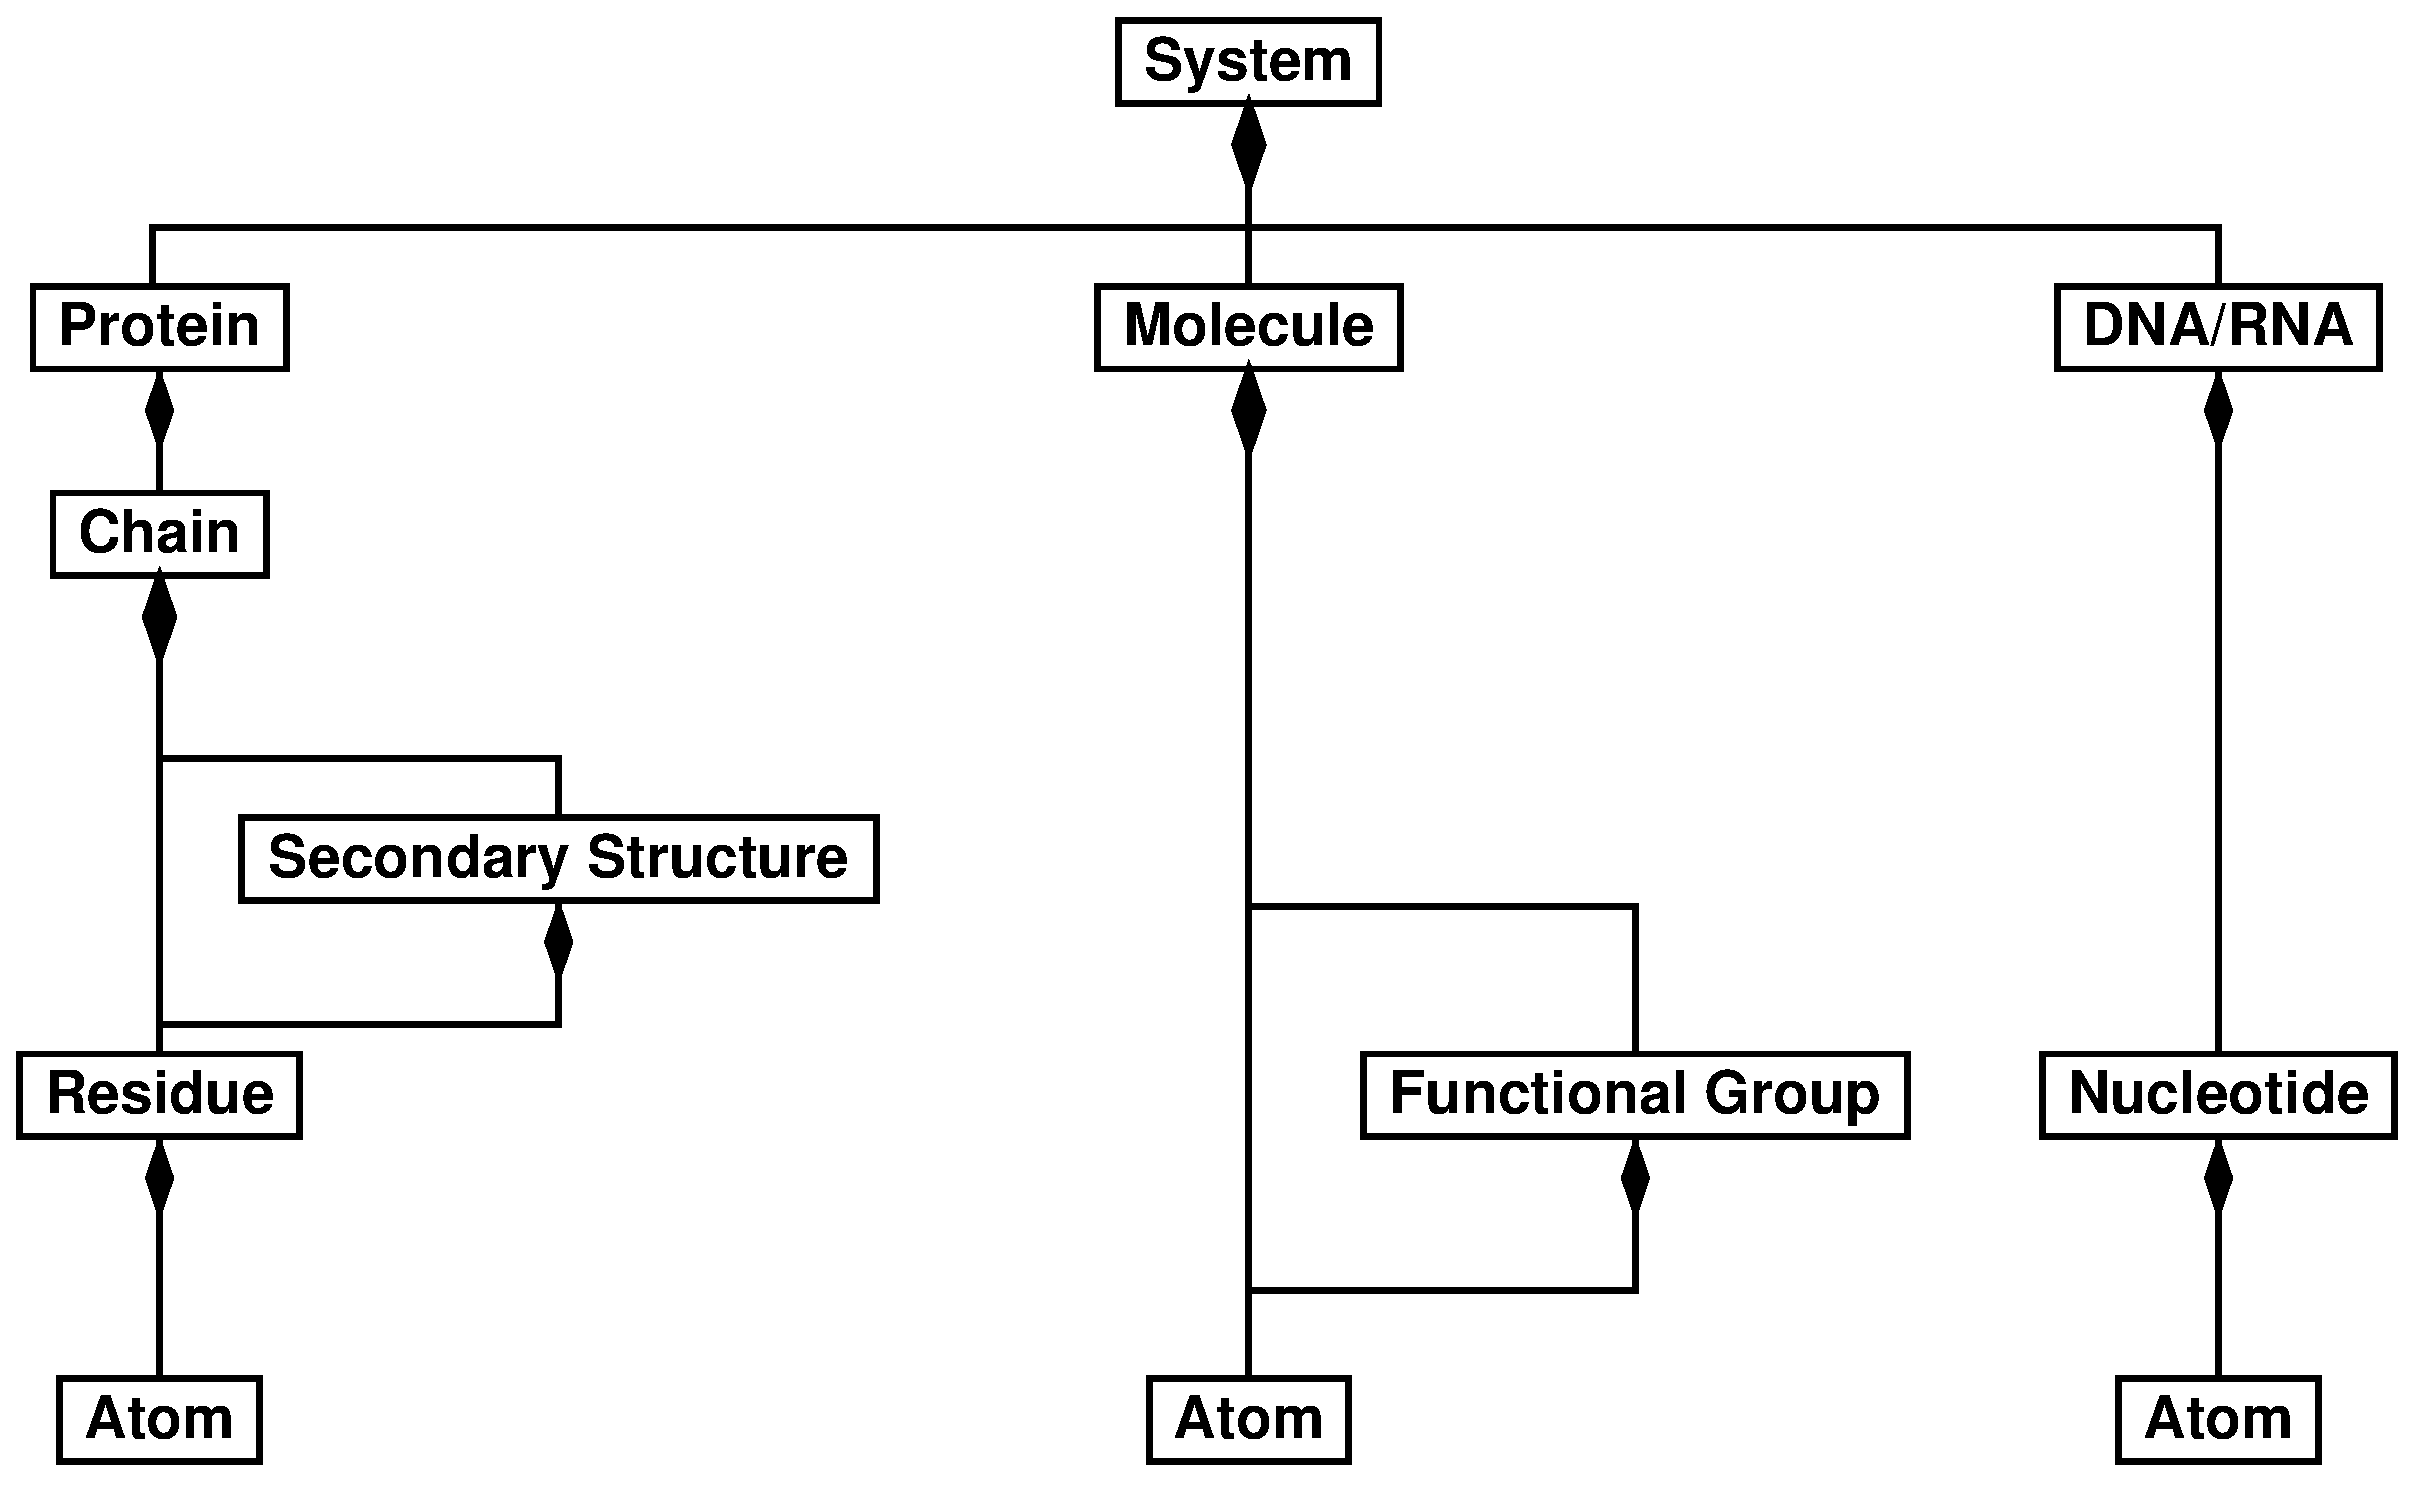
\includegraphics[width=\textwidth]{problem-domain.eps}
  \caption{A model of the biochemical problme domain. BALL tries to model
					these entities as closely as possible with its kernel classes.}
  \label{figure:problem-domain}
\end{figure}

\begin{figure}[tb]
  \centering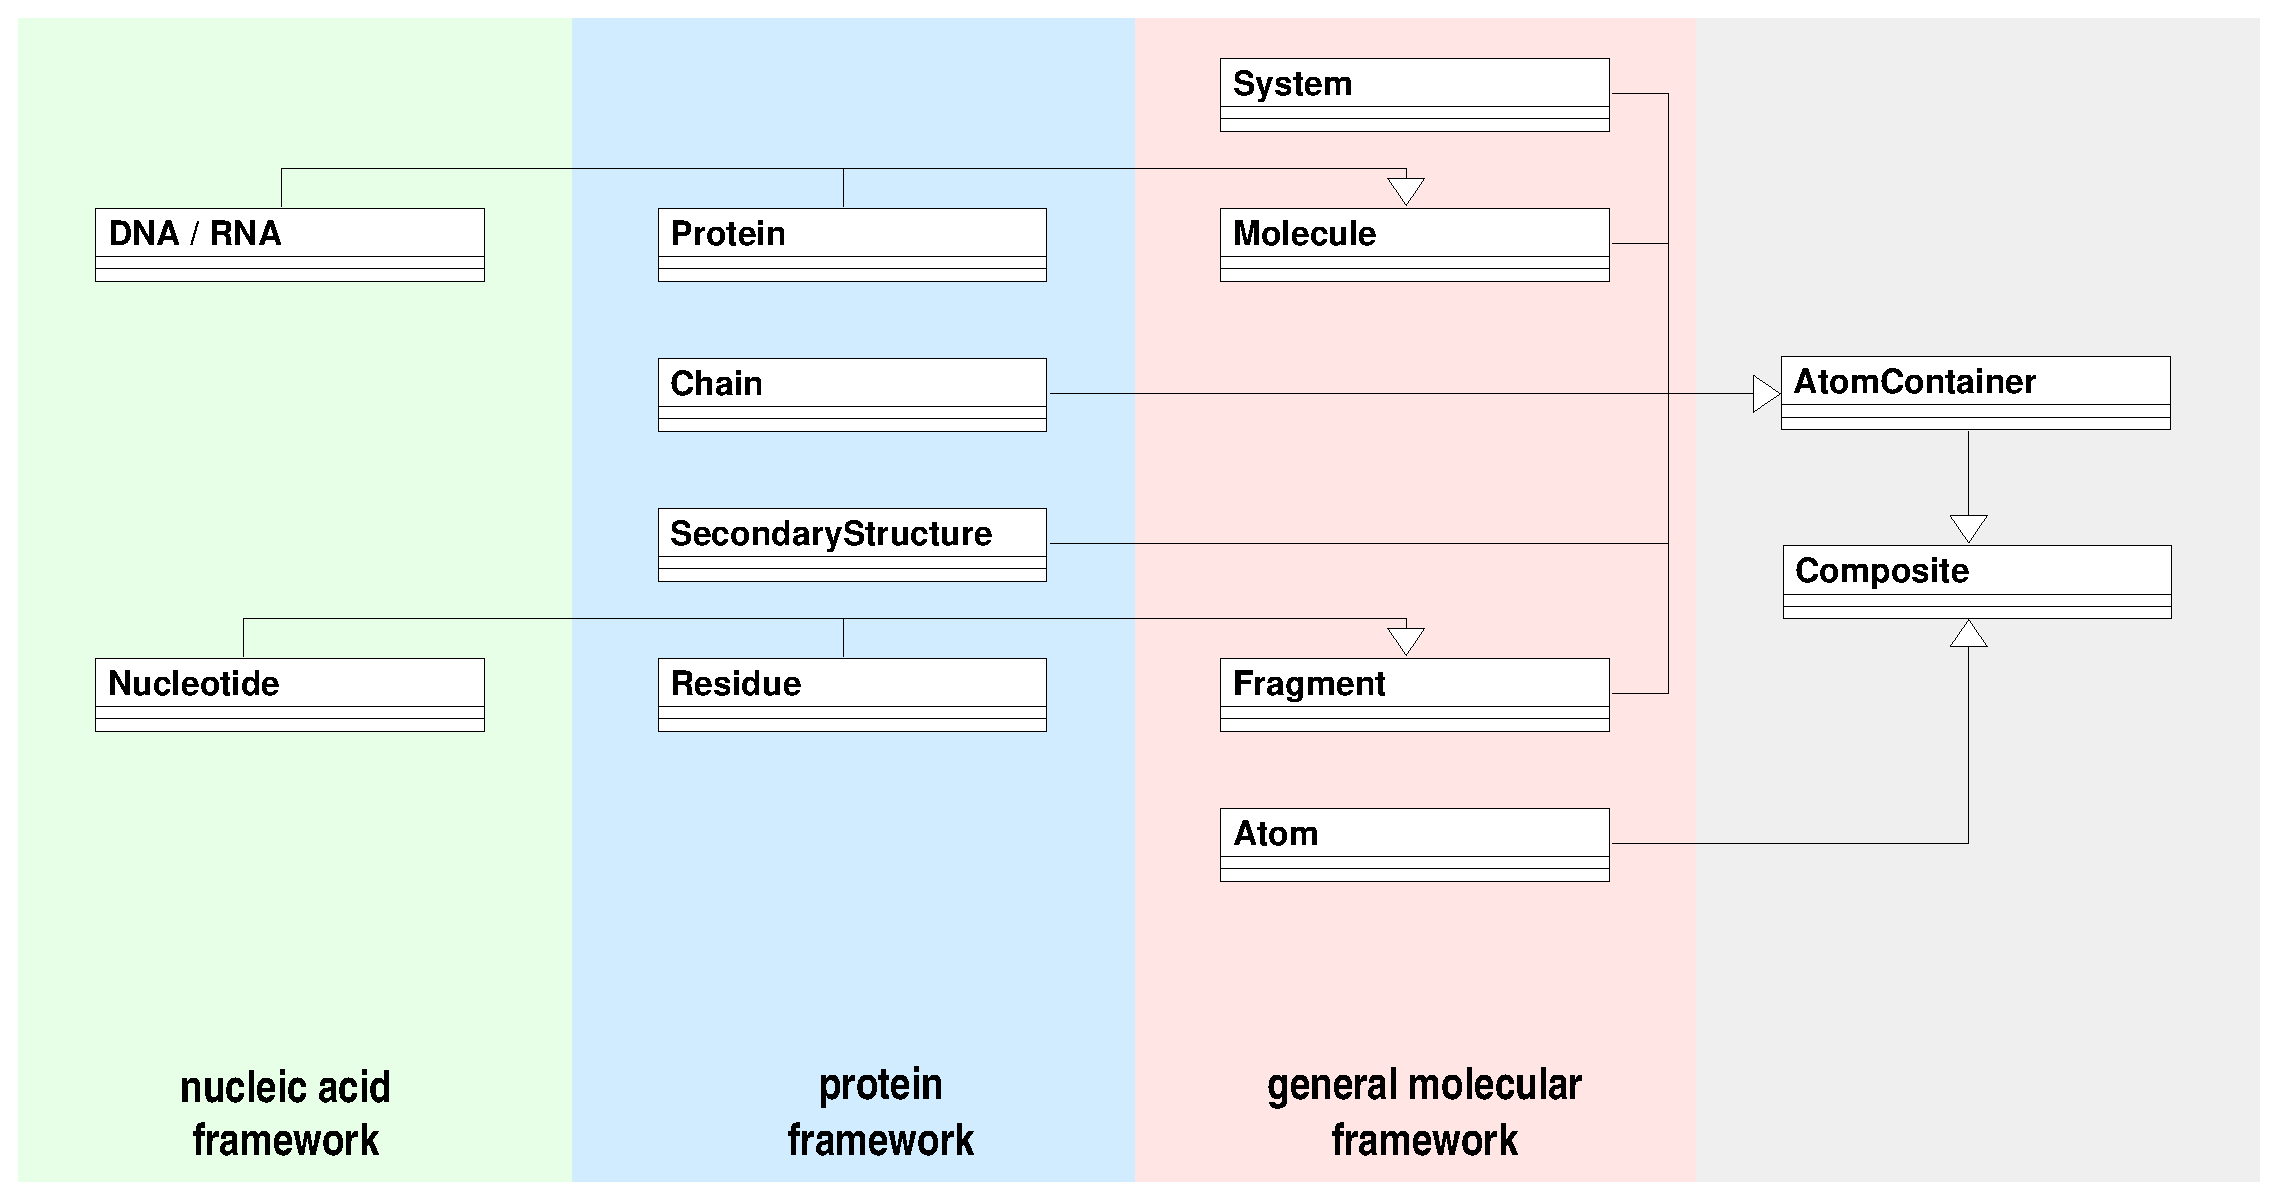
\includegraphics[width=\textwidth]{kernel-data-structures.eps}
  \caption{The BALL kernel classes consist of three main frameworks: the
molecular framework, the protein framwork, and the nucleic acid framework.}
  \label{figure:kernel-frameworks}
\end{figure}

\paragraph{The molecular framework} contains the classes \class{System},
\class{Molecule}, \class{Fragment}, \class{Bond}, and \class{Atom}. 
Molecules can contain an arbitrary number of atoms or fragments. A fragment
can be used to define distinct groups in a molecule, \eg functional groups or
charge groups. Fragments can be nested, so you may want to define several
functional groups within one larger fragment in a molecule. The atoms are then
contained in the fragments. In contrast to other systems, the atoms of a
molecule are not necessarily connected to each other (or in graph-theoretical
terms: they do not have to represent a connected component of the graph
formed by atoms and bonds). Systems are nothing but collections of molecules.

\paragraph{The protein framework} is a specialization of the general molecular
framework and describes the structures encountered in proteins. Proteins are
(more or less) molecules, so \class{Protein} is a subclass of \class{Molecule}
and proteins can be handled like molecules and stored along with them in
systems. Proteins can often be decomposed into several chains. These chains in
turn can contain secondary structure elements, which then contain residues.
Residues usually describe the amino acids of a protein. THe sequence
information of a protein is encoded implicitly in the order of the tree: it
can be obtained by reading all instances of \class{Residue} in the order they
are contained in a protein. So the protein, the chains, and secondary
structure elements should contain the residues in the correct order, from
N-terminal to C-terminal, if you construct them by hand. The first and last
residue of a chain are considered to be terminal (according to the member
function \member{Residue}{isTerminal}). This is also the reason why a protein
should always contain at least one chain. Secondary structure elements,
defined by \class{SecondaryStructure} are optional. Wherever this information
is known (\eg when read from PDB files), instances of
\class{SecondaryStructure} are created to store it. Each secondary structure
element contains a class {\eg helix, $\beta$-sheet) describing its type.

\paragraph{The nucleic acid framwork} contains the classes \class{NucleicAcid}
and \class{Nucleotide} and is used to represent structures of nucleic acids.
Right now, we do not differentiate between DNA and RNA, so if you need these
classes, we are eager to get your input on how to model DNA and RNA in a more
detailed way -- currently do not have yet any application for it.

By deriving all kernel classes from the commonn base class \class{Composite},
they share all the features implemented there. The following section will
briefly discuss some of these features.

\paragraph{Iteration} over kernel data structures is a key concept in BALL.
The BALL kernel iterators a re STL-like iterators. Since most BALL kernel
classes are so-called {\em multi-containers}, \ie they can contain different
objects, we cannot use the typical STL {\tt begin()}/{\tt end()} methods.
For example in a protein, you might not only want to iterate over all chains,
but also over all residues or all atoms contained therein. So in BALL there
are the methods \member{System}{beginChain()}/


\chapter{VIEW Programming}
\label{chapter:view-programming}
\noindent
Visualization not only covers the graphical representation of things (\eg
molecules, measurement data, \dots) but also the graphical user interface
(GUI). Both jobs can be done using \class{VIEW} functionality. Both areas are
discussed in the next few sections.

\section{Modularity}
In general most of the time in GUI programming is spent on implementing the 
interactions of the individual elements of the user interface with each other 
(\eg defining menu entries, button actions, etc.). In order to reduce these 
efforts, the functionality in the VIEW library has been bundled into different
modules (\eg OpenGL rendering, force field methods, the scripting language 
interface, etc.), which can be freely combined to an application. These modules
automatically connect to each other and thus allow the user to add further 
functionality with as little as a single line of code. To this end, we have 
designed a set of  base classes describing the interactions of the interface 
elements. The two most important components in this design are 
\class{MainControl}, the application's main window, and 
\class{ModularWidget}, the base class for all modules.
The next pages will describe the modeling and implementation of this approach.
\label{modularity}

\paragraph{MainControl} 
\hspace*{\fill}\\
The class \class{MainControl} is derived from Qt's \class{QMainWindow} and thus
realizes an application's main window. It contains only the most essential data
structures: The \class{CompositeManager} stores all molecular entities
(\class{Composite} objects) and the \class{PrimitiveManager} is responsible for
the representations (\ie geometric models) and the thread for their
(re)calculation. All additional functionality (\eg reading and writing of 
structures, OpenGL visualization, etc.) are added to the main window by 
instantiating one of the classes derived from \class{ModularWidget}. 

\paragraph{Modular Widgets}
\hspace*{\fill}\\
\class{ModularWidget} is a common base class for all the modules, that can be
combined to form an entire application. While the modular widgets are widely 
independent, they can still notify each other about the current work flow. 
This is achieved by a messaging system, that allows a \class{ModularWidget}
to send a message which is then received by all other modular widgets (see 
Section~\ref{message}).
\\
In addition to the messaging system, the \class{ModularWidget} class provides 
many other commonly needed features to ease and accelerate the development of
new modules:
\begin{itemize}
%\item Sending and receiving of messages
  \item Showing status and error messages
  \item Management of menu and toolbar entries 
  \item Registering widgets and menu entries for the help system
  \item Management of preferences dialogs
  \item Reading/writing of settings from/to a configuration file
  \item Registering of supported file formats \eg for parsing command line
        arguments or drag-and-drop support
  \item Access to individual instances with the method \class{getInstance()}
  \item Access to the \class{MainControl} and thus to the loaded molecules and
        representations
  \item Locking of molecular entities while multithreaded code is running
\end{itemize}

For many different tasks (see Table \ref{table:tmw}),
the VIEW library already contains a wide variety of modular widgets.
Since they are widely independent from each other, they can easily
be combined to an application. All that is needed, is the instantiating
of modular widgets with the \class{MainControl} as their parent, as can be seen in
the following code snippet:
\begin{lstlisting}{}
Mainframe::Mainframe(...)
  : MainControl(...)
{
  new LogView(this);          // widget (1)
  new DatasetControl(this);   // widget (2)
  new PyWidget(this);         // widget (3)
  new MolecularControl(this); // widget (4)
  new GeometricControl(this); // widget (5)
  new Scene(this);            // widget (6)
}
\end{lstlisting}

These few lines of code (header includes were omitted for brevity) create a fully-fledged 
molecular structure viewer.
In addition to using already existing widgets, users can easily implement new ones,
especially since \class{ModularWidget} already offers many common features (see above).
As a result, users can freely combine new and existing widgets both 
to extend BALLView with new functionality or to create entirely new custom-tailored 
applications.

\begin{table} [ht] %[htbp]
\centering
\begin{tabular} {|l|l|}
\hline
\bf Name                            & \bf Functionality\\
\hline
\class{DatasetControl}              & Management of data sets\\
\class{DisplayProperties}           & Creation and modification of models\\
\class{DockingController}           & Molecular docking\\
\class{DownloadPDBDialog}           & Downloads from the protein database\\
\class{EditableScene}               & Molecular editing\\
\class{FDPBDialog}                  & Calculation of electrostatic potentials\\
\class{FileObserver}                & Observing changes in a molecular file\\
\class{GeometricControl}            & Management of graphical representations\\
\class{LabelDialog}                 & Creation of labels in the 3D view\\
\class{LogView}                     & Logging window\\
\class{ModifyRepresentationDialog}  & Custom colorings for models\\
\class{MolecularControl}            & Hierarchical overview of loaded
                                      molecules\\
\class{MolecularFileDialog}         & Reading and writing of molecular files\\
\class{MolecularStructure}          & Force field and molecular mechanics
                                      features\\
\class{PyWidget}                    & Python scripting\\
\class{Scene}                       & three-dimensional graphics\\
\class{SnapshotVisualisationDialog} & Visualization of trajectories\\
\class{TestFramework}               & Recording and playback of user input\\
\hline
\end{tabular}
\caption[Overview on the derived modular widgets]
{Overview of the classes derived from \class{ModularWidget}. 
Each individual class was created for one specific domain of features and is widely 
independent from the other widgets.
}
\label{table:tmw}
\end{table}


\paragraph{Example for the implementation of a modular widget}
\hspace*{\fill}\\
To visualize how new modular widgets can be created, the following pages will outline 
the implementation of the class \class{LabelDialog}, which is
part of the VIEW library. 
Its purpose is to create labels in the 3D view for a list of 
highlighted molecular entities and it has the following capabilities:
The menu entry {"Add Label"} toggles the dialog's visibility and is 
disabled if no molecular entities are highlighted in the \class{MolecularControl}.
When the dialog is shown, the user can select a font and its color, the desired text for 
the label(s), and choose if only one label is to be created for the entire selection or 
one label for every atom/residue.  
When the "Apply" button is pressed, a new \class{Representation} is created with the newly 
created label(s).
For convenience the chosen color and font are stored in the application's configuration 
file for future usage.
\\ 
\\
The dialog's layout was done with the program "Qt Designer" (see ~\ref{designer}).
This results in a source file, containing the base class \class{Ui\_LabelDialogData}, which 
defines the dialog's layout. The actual dialog class is derived from this layout class.
This procedure accelerates the development process and makes the dialog's 
layout independent from its function.
The following code is the content of the header file for the actual dialog.
The includes, namespaces, and some documentation lines were omitted for brevity and the
overloaded methods from the \class{ModularWidget} base class were marked.
\begin{lstlisting}{}
class BALL_VIEW_EXPORT LabelDialog 
  : public QDialog,
    public Ui_LabelDialogData,
    public ModularWidget
{
  // macro needed for Qt's slot mechanism:
  Q_OBJECT

  // Macro from the Embeddable class:
  BALL_EMBEDDABLE(LabelDialog,ModularWidget)
	
  public:
  LabelDialog(QWidget *parent = NULL, const char *name = NULL );
  virtual ~LabelDialog();
					
  // method for message handling, overloaded from ModularWidget
  virtual void onNotify(Message* message);
					
  // method for reading settings, overloaded from ModularWidget
  virtual void fetchPreferences(INIFile &inifile);
  // method for written settings, overloaded from ModularWidget
  virtual void writePreferences(INIFile &inifile);
		
  // method for e.g. initializing menu entries, overloaded from ModularWidget
  virtual void initializeWidget(MainControl& main_control);

  // Overloaded from ModularWidget
  virtual void checkMenu(MainControl& main_control);
	
  protected slots:
  virtual void accept();
  virtual void editColor();
  virtual void addTag();
  virtual void fontSelected();
  virtual void modeChanged();
  void textChanged();

  protected:
  Representation* createOneLabel_();
  Representation* createMultipleLabels_();
  QAction*    menu_entry_;
  ColorRGBA   custom_color_;
  QFont       font_;
};
\end{lstlisting}

The following paragraphgraphs will discuss the actual implementation, starting with the 
constructor: It must be called with the \class{MainControl} as parent to enable the 
registration of the \class{ModularWidget}.
Since this example class is derived from three other classes, these also have to
be initialized. 
The function \class{setupUi} stems from the ''*.ui' file and defines the layout of the dialog.
Next the individual buttons and check boxes are connected to their slots.
The call of \class{registerWidget} is of special importance since it enables the internal 
mechanism that connects all modular widgets with each other (i.e.\ the messaging system).
\begin{lstlisting}{}
LabelDialog::LabelDialog(QWidget* parent, const char* name)
  :  QDialog(parent),
     Ui_LabelDialogData(),
     ModularWidget(name)
{
  // apply the dialogs layout:
  Ui_LabelDialogData::setupUi(this);

  // signals and slots connections
  connect(apply_button_, SIGNAL(clicked()), this, SLOT(accept()));
  connect(buttonCancel, SIGNAL(clicked()), this, SLOT(reject()));
  connect(edit_button, SIGNAL(clicked()), this, SLOT(editColor()));
  connect(add_tag_button, SIGNAL(clicked()), this, SLOT(addTag()));
  connect(font_button, SIGNAL(clicked()), this, SLOT(fontSelected()));
  connect(all_items, SIGNAL(toggled(bool)), this, SLOT(modeChanged()));
  connect(text_box, SIGNAL(editTextChanged(const QString&)), 
              this, SLOT(textChanged()));

  setWindowTitle("Add Label");
  setObjectName(name);
  hide();

  // register the widget with the MainControl
  ModularWidget::registerWidget(this);
}
\end{lstlisting}

All modular widgets can have their own menu entries in the applications menu bar.
These entries should be initialized in the virtual method 
\class{initializeWidget}, which will be automatically called by the \class{MainControl}
for all registered \class{ModularWidget} subclasses.
For this concrete class, the method creates the menu entry "Add Label" and connects 
it to a slot, which will open the dialog. 
The creation of the menu entry is done through a call of \class{insertMenuEntry}, 
which will also create the given menu (if it does not yet exist) and return a pointer to 
a \class{QAction}. 
This pointer is then assigned to the variable \class{id\_}, which will later be used for 
enabling and disabling the menu entry.
Corresponding to the method \class{initializeWidget} exists the \class{initializePreferencesTab} method to add sub pages to the applications preferences dialog. 
Since this dialog does not have a configuration dialog, this function is not needed in 
the \class{LabelDialog} class.
\begin{lstlisting}{}
void LabelDialog::initializeWidget(MainControl& main_control)
{
  menu_entry_ = ModularWidget::insertMenuEntry(
                  MainControl::DISPLAY, "Add Label", this, SLOT(show()));
  setMenuHint("Add a label for selected molecular objects");   
}
\end{lstlisting}

\vspace{-0.2cm}
The next method \class{onNotify} does the message processing:\label{onNotify}
It is overloaded from the \class{ModularWidget} class and gets called when a \class{Message} 
arrives for the widget. In the \class{LabelDialog} class, it does the following:
If no molecular entities are highlighted in the \class{MolecularControl}, the dialog's 
"Apply" button is disabled and the menu entries are checked if they have to be 
enabled/disabled. 
This is done to ensure, that the dialog can not be used while \eg a simulation is 
running, since the molecular entities could changed at any time. 
This is checked in the \class{checkMenu} method with a call to \class{MainControl::isBusy()}, 
which returns true if a modular widget locked the molecular entities because they could 
be changed or if an model update is underway.
\begin{lstlisting}{}
void LabelDialog::onNotify(Message* message)
{
  ControlSelectionMessage* sm = 
    RTTI::castTo<ControlSelectionMessage>(*message);

  if (sm != 0)
  {
    // disable apply button, if selection is empty
    apply_button_->setEnabled(!sm->getSelection().empty();
    checkMenu(*getMainControl());
  }
}

void LabelDialog::checkMenu(MainControl& mc)
{
  Size selection_size = mc.getMolecularControlSelection().size();
  menu_entry_->setEnabled(selection_size && !mc.isBusy());
}
\end{lstlisting}

The following methods are only of minor interest and just shown for the sake of completeness.
They are called when a user clicks on the
corresponding buttons and perform auxiliary functions, like choosing the label's 
font or color.
\begin{lstlisting}{}
void LabelDialog::editColor()
{
  custom_color_.set(chooseColor(color_sample_));
}

void LabelDialog::addTag()
{
  QString tag;
  if (tag_box->currentText() == "Name")                tag = "%N";
  else if (tag_box->currentText() == "Residue ID")     tag = "%I";
  else if (tag_box->currentText() == "Atom Type")      tag = "%T";
  else if (tag_box->currentText() == "Atom Charge")    tag = "%C";
  else if (tag_box->currentText() == "Atom Type Name") tag = "%Y";
  else if (tag_box->currentText() == "Element")        tag = "%E";

  text_box->lineEdit()->setText(text_box->currentText() + tag);
}

void LabelDialog::fontSelected()
{
  bool ok = true;
  QFont font = QFontDialog::getFont(&ok, font_, 0);
  if (!ok) return;

  font_label->setFont(font);
  font_ = font;
}

void LabelDialog::modeChanged()
{
  tag_box->setEnabled(!all_items->isChecked());
  add_tag_button->setEnabled(!all_items->isChecked());
}

void LabelDialog::textChanged()
{
  apply_button_->setEnabled(text_box->currentText() != "");
}
\end{lstlisting}

\vspace{0.5cm}
When a user presses the dialog's "Apply" button, the method \class{accept()} is called.
It does the actual label creation and adds the label(s) to the 3D view:
First the current list of highlighted molecular entities is obtained from
the \class{MainControl}.
Then a \class{LabelModel} processor is created and added to a \class{Representation}.
Next the values from the dialog are applied to the \class{LabelModel} and the
list of molecular entities is stored in the \class{Representation}.
This approach may seem a bit complex but it has a distinct advantage: The position
of the label will be automatically updated if the 3D positions of the molecular entities 
should change. 
Finally the \class{Representation} is stored in the \class{MainControl} and it is rendered
in the 3D view with a call of \class{MainControl::update(Representation\&)}.
The methods in the \class{MainControl} for inserting and updating representations were 
added just for convenience reasons and contain only the code for sending the corresponding 
messages. 
As an example, \class{MainControl::insert(Representation\&)} only consists of the 
following code:
\begin{lstlisting}{}
  notify_(new RepresentationMessage(representation, 
                                    RepresentationMessage::ADD));
\end{lstlisting}

After the last modular widget was notified, the message will be automatically deleted.
Therefore messages, that are about to be send, have to be created on the heap.
\begin{lstlisting}{}
void LabelDialog::accept()
{
  List<Composite*> selection = 
    getMainControl()->getMolecularControlSelection();

  // no selection present => return
  if (selection.empty()) return;

  Representation* rep = new Representation;
  rep->setProperty(Representation::PROPERTY__ALWAYS_FRONT);
  rep->setModelType(MODEL_LABEL);

  LabelModel* model = new LabelModel;
  model->setText(ascii(text_box->currentText()));
  model->setColor(custom_color_);
  model->setFont(font_);

       if (    all_items->isChecked()) model->setMode(LabelModel::ONE_LABEL);
  else if (   every_atom->isChecked()) model->setMode(LabelModel::ALL_ATOMS);
  else if (every_residue->isChecked()) model->setMode(LabelModel::ALL_RESIDUES);
  else if (   every_item->isChecked()) model->setMode(LabelModel::ALL_ITEMS);

  rep->setModelProcessor(model);

  // process all objects in the selection list
  List<Composite*>::ConstIterator list_it = selection.begin();
  List<const Composite*> composites;
  for (; list_it != selection.end(); ++list_it)
  {
    composites.push_back(*list_it);
  }

  rep->setComposites(composites);
  getMainControl()->insert(*rep);
  getMainControl()->update(*rep);
  text_box->addItem(text_box->currentText());
  setStatusbarText("Label added.");
}
\end{lstlisting}

The next two methods are responsible for reading and writing the of this widget's settings.
The first method, \class{fetchPreferences}, restores the settings from the configuration file.
If the this file has a section with the name \class{WINDOWS} and a key 
''\class{Label::customcolor}'' within, then the content of this key is read and converted 
to a color, which is then assigned to the dialog's label and stored in the variable
\class{custom\_color\_}.
\begin{lstlisting}{}
void LabelDialog::fetchPreferences(INIFile& inifile)
{
  // restore the color 
  if (inifile.hasEntry("WINDOWS", "Label::customcolor"))
  {
    custom_color_.set(inifile.getValue("WINDOWS", "Label::customcolor"));
    setColor(color_sample_, custom_color_);
  }

  // restore the font
  if (inifile.hasEntry("WINDOWS", "Label::font"))
  {
    font_.fromString(inifile.getValue("WINDOWS", "Label::font").c_str());
  }
  font_label->setFont(font_);
}
\end{lstlisting}

\vspace{0.3cm}
To write all user defined options in a configuration file, the method
\class{ModularWidget::writePreferences} was overridden:
\begin{lstlisting}{}
void LabelDialog::writePreferences(INIFile& inifile)
{
  ModularWidget::writePreferences(inifile);

  // store the color
  inifile.insertValue("WINDOWS", "Label::customcolor", custom_color_);
  // store the font
  inifile.insertValue("WINDOWS", "Label::font", ascii(font_.toString()));
}
\end{lstlisting}

This concludes the implementation of the \class{LabelDialog} class. 
It can be used in a derived \class{MainControl} class, simply by adding the following line: 
\begin{verbatim}
	new LabelDialog(this, "LabelDialog");
\end{verbatim}
This one line of code is all that is needed to make the dialog work, all needed function 
calls inside the \class{LabelDialog} class will be automatically done by the VIEW framework.
\\
\\
This example demonstrates, how effective the encapsulation of features into distinct
modules works: Since the modules are mostly independent from each other and the interface
base classes take care of all basic functions, it is very easy to extend the application
with new features.

\section{Messaging system} \label{message}
A special mechanism was needed for allowing the individual modular widgets to be mostly 
independent from each other but still be able work together i.e.\ by notifying each other 
about the current work flow. 
This was achieved by a messaging system, that allows a \class{ModularWidget} to send a 
message which is then received by all other modular widgets.
As an example: 
The \class{MolecularControl} provides a hierarchical overview of the loaded molecules
and notifies the other widgets when a user highlights some of its entries. 
This is needed, since other modular widgets offer tool bar entries for features (like 
saving molecules) that operate on the currently highlighted objects. 
These entries get disabled if no molecular item is highlighted.
To notify the other widgets, the \class{MolecularControl} sends a \class{ControlSelectionMessage}
which is then received by the \class{MolecularFileDialog}.
This class provides the functionality for loading and writing molecular files and will 
then disable the corresponding menu and toolbar entries.\\
Since the modular widgets have to notify each other about many different events, the class
\class{Message} has many subclasses (see Table~\ref{tab:messages}), which store different data
types, like selections or object pointers. 
If a new event is introduced, it can easily be added by creating an other \class{Message} 
subclass.
\\
The actual sending of messages is done in the method \class{ModularWidget::notify\_}, while 
the message is received by \class{ModularWidget::onNotify()} (for an example of a concrete
implementation see page~\pageref{onNotify}).
In this method the modular widget has to decide if it needs to react to the message. 
This is in general done by using runtime type identification. 
In addition, many different messages also provide enumeration values for defining further
specialized message subtypes. 
A \class{CompositeMessage} can \eg cope with the events of an added or deleted 
\class{Composite} by using the types \class{CompositeMessage::NEW\_COMPOSITE} or 
\class{CompositeMessage::REMOVED\_COMPOSITE}.
The usage of these enumeration subtypes has the advantage, that much less subclasses
are needed to distinguish different classes of events, resulting in a slimmer implementation.
Thus we only added new \class{Message} subclasses, when a message had to transmit a new kind 
of data, or if no appropriate class yet existed.
%-- Anordnung der Casts entsprechend der auftretenden Hauefigkeit der Nachricht\\
%The current implementation has a small drawback: Since all modular widgets receive a message
%the method onNotify() may be called many times in a row. 
\begin{table} [ht] %[htbp]
\centering
\begin{tabular} {|l|l|}
\hline
CompositeMessage & SceneMessage\\
GenericSelectionMessage & ControlSelectionMessage\\
NewSelectionMessage & GeometricObjectSelectionMessage\\
RepresentationMessage & MolecularTaskMessage\\
ShowDisplayPropertiesMessage & CreateRepresentationMessage\\
RegularDataMessage & RegularData1DMessage \\
RegularData2DMessage & RegularData3DMessage\\
NewDockResultMessage & NewTrajectoryMessage\\
ShowDockResultMessage & DockingFinishedMessage\\
DeselectControlsMessage & \\
\hline
\end{tabular}
\caption{Derived message classes. 
All the individual classes can contain specific datas and some have an addition enumeration 
type to differ between subtypes of messages.}
\label{tab:messages}
\end{table}
%
\section{Design of the visualization classes}
\paragraph{Geometric objects}
\hspace*{\fill}\\
\label{geometric_objects}
We created a base class \class{GeometricObject} to provide a general interface
for geometric shapes, that can be calculated and rendered in the VIEW
framework. From this base class, we then derived the classes for the individual
tangible geometric objects (see Table~\ref{tab:go}). The instances of these 
derived classes are created by the different model processors and later get 
colored by the color processors, and stored in a \class{Representation}. The 
renderer classes can then translate their informations such that they can \eg
be drawn on the screen or processed by an external program.
\begin{table} [ht] %[htbp]
\centering
\begin{tabular} {|l|l|}
\hline
Box & Disc\\
Label & GridVisualisation\\
Mesh & QuadMesh\\
Point & SimpleBox\\
Sphere & Tube\\
Line & TwoColoredLine \\
Tube & TwoColoredTube\\
IlluminatedLine& \\
\hline
\end{tabular}
\caption{Overview of the different geometric objects that are supported in the VIEW 
	framework.}
\label{tab:go}
\end{table}

We created numerous derived \class{GeometricObject} classes, to guarantee that virtually
all thinkable shapes and objects can be visualized. 
If nevertheless in the future the need for a new kind of geometric object would arise, 
this could be realized with minimal effort:
All that would have to be done, is to create a new derived \class{GeometricObject} class and 
add the corresponding rendering methods to the \class{Renderer} classes 
(see Page~\pageref{renderer}).

\label{representation}
\paragraph{Representations}
\hspace*{\fill}\\
To offer the user an intuitive way of handling models and their coloring,
we created the class \class{Representation}. 
For each visualized object, this class stores the selection of molecular entities, the used 
model and coloring method, the drawing style, and the geometric objects representing the 
model (see Fig.~\ref{fig:representation}).
This approach has many advantages:
\begin{itemize}
  \item The different models and coloring methods can be freely combined.
  \item Users can can create customized representations \eg by using the Python
        scripting interface.
  \item Users can combine as many different representations as they like to
        compose complex molecular visualizations.
  \item Individual representations can be enable/disable any time.
  \item It is possible to write project files, which store all representations
        for later usage.
  \item A \class{Representation} can easily be redrawn, when the corresponding
        atoms have changed.
  \item A user can disable all updates to a representation \eg to visualize the
        differences between two steps in a trajectory.
\end{itemize}

We wanted to make the creation and modification of representations as easily as possible.
Thus we designed a user friendly dialog, which can assign all
the different settings of a \class{Representation}.\\
The classes \class{ModelProcessor} and \class{ColorProcessor} which are responsible 
for creating the different models and coloring schemes are described in the
section below.
\begin{figure*}[ht] %[htbp]
\centering
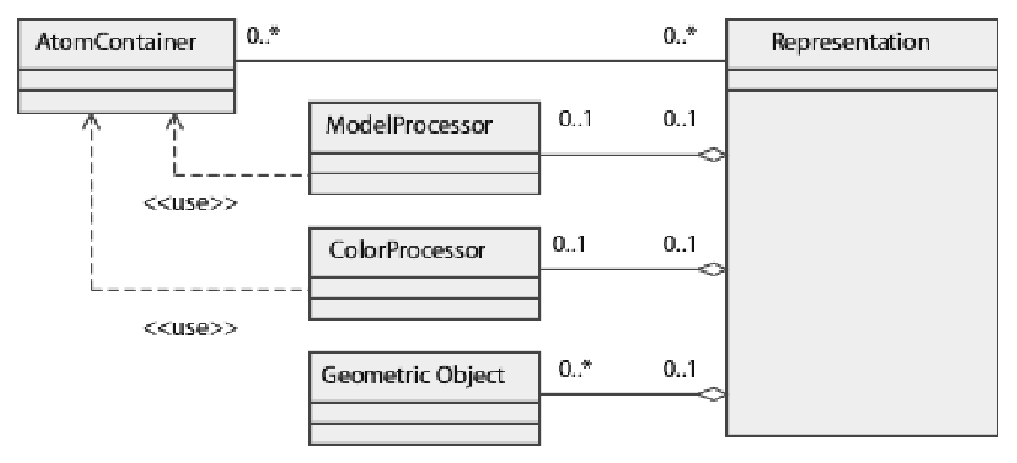
\includegraphics[width=1.\textwidth]{representation.eps}
\caption[UML diagram for the \class{Representation} class]
{Each visualized object corresponds to an instance of the class 
\class{Representation}. The \class{ModelProcessor} creates 
\class{GeometricObjects}, \eg tubes or meshes for all atoms stored in the
\class{AtomContainers}. Next, the \class{ColorProcessor} colorizes the 
\class{GeometricObjects}, \eg by element, charge or temperature factor. The
individual model types and coloring methods are realized by derived classes.
This approach simplifies the creation of new models and coloring methods and 
allows their free combination.}
\label{fig:representation}
\end{figure*}

\paragraph{Models and Coloring}
\hspace*{\fill}\\
We created a wide variety of different models.
All these model classes are derived from the \class{ModelProcessor}.
This class is again derived from the BALL class \class{UnaryProcessor$<$Composite$>$}, 
which provides a general interface for recursively iterating and processing a 
\class{Composite} tree.
Therefore a \class{ModelProcessor} can be be applied to entire proteins as well as on 
individual atoms, which makes it is easily possible to create models for user defined 
subselections of molecules.
When a model processor is applied to such a selection, it first iterates over the
\class{Composite} tree and collects the information necessary for the model's creation.
With this information, the method \class{createGeometricObjects()} can then create the 
individual geometric object, which form the model. 
The geometric objects are created on the heap and stored in a list inside the 
\class{Representation}, which is then responsible for deleting them.
\\
The counterpart to \class{ModelProcessor} is \class{ColorProcessor}, which iterates over a 
list of \class{GeometricObjects} and finds the corresponding color for each one.
Currently 16 different coloring methods are implemented and
every single one is derived from \class{ColorProcessor}.
\\
Since users directly perceive on how long it takes to create a representation,
we made great efforts to ensure maximum performance for the model and coloring 
calculations.

\paragraph{Renderer}\label{renderer}
\hspace*{\fill}\\
Currently BALLView support two different renderer: Real time graphics are provided by the
OpenGL renderer (\class{GLRenderer}) while high quality graphics are available through the 
POVRay exporter (\class{POVRenderer}).
Both classes are derived from a common base class \class{Renderer}, which provides a general 
interface.
This ensures, that in future versions, arbitrary renderer can easily be added by
deriving a further class from \class{Renderer}.
The actual rendering of a \class{Representation} is done in the method
\class{Renderer::render(const Representation\&)}.
It iterates over all geometric objects in the \class{Representation} and,
by using runtime type identification, finds the corresponding rendering method:
\begin{lstlisting}{}
  if      (RTTI::isKindOf<Point>(*go))
            renderPoint_(*(const Point*) go);
  else if (RTTI::isKindOf<Disc>(*go))
            renderDisc_( *(const Disc*)  go);
  else if (RTTI::isKindOf<Line>(*go))
            renderLine_( *(const Line*)  go);
\end{lstlisting}
 
These methods are overridden in the derived classes with the real rendering
code, \eg OpenGL calls in the \class{GLRenderer}. 
This approach ensures that the different renderer can easily be extended with support for 
new kinds of geometric objects, simply by adding a new rendering method and an appropriate 
runtime check.

Unlike the OpenGL renderer, the \class{POVRenderer} does not provide real time graphics,
but an interface to the external POVRay renderer.
To do so, it translates the data in the geometric objects to a form that can be 
parsed by the POVRay application. 
The resulting text is then written to an output stream, which is either a
file or the standard console output.

\section{Creating dialogs}
\label{designer}
To layout the dialogs in the VIEW library, we used the program "Qt Designer".
It is part of every Qt-package and provides a comfortable "What you see is what you get"
(WYSIWYG) interface for designing widgets.
The result of the "Qt Designer" program is a ".ui" file, which is then transformed 
into a set of C++ source files by the Qt program "uic".
These source files contain a base class, which defines the dialog's layout . 
The actual dialog class will be derived from the layout class and contains the dialog's
actual functionality.

While this procedure may seem a bit complicated, it is actually straightforward and 
very useful:
Not only does the "Qt Designer" WYSIWYG interface accelerates the development process, 
the resulting "*.ui" files also uncouple the dialogs' layout from its function. 
Thus a software engineer can extend the functionality without 
having to care about the dialog's layout, while a GUI designer can change the layout
without the need to adapt the source code.

\section{User defined settings}
\label{preferences}
We wanted to give BALLView's users the opportunity to adapt it to their liking in any
thinkable way, including the different models, coloring methods, and display options. 
Therefore an extensible graphical user interface was needed for applying these settings. 
For this purpose, we developed the \class{Preferences} dialog, which can contain an 
arbitrary number of child dialogs. 
These child dialogs are stored in a \class{QWidgetStack} and shown as entries in 
a hierarchical list. 
If a user clicks on such an entry, the corresponding dialog is then shown in the 
widget stack.
This approach allows to cluster the different settings in a hierarchical way
and users can freely browse and apply the individual settings.
Furthermore the \class{Preferences} dialog can have any number of child dialogs and still 
have a concise layout.
In an earlier implementation, we used a tab widget, which is the standard approach for
such dialogs. This solution proved to be less suited, since the child dialogs can not
be clustered and the layout becomes unhandy, if many children are added.

\paragraph{Automation of the (re)storing process}
\hspace*{\fill}\\
All the settings, that can be adapted in the \class{Preferences} dialog, shall be 
stored when BALLView is closed.
To this end all configuration dialogs have to store the content of their GUI elements,
like line edits or check boxes.
In the early versions of our implementation, every dialog provided its
own routines for this purpose.
Since this created a lot of overhead in means of redundant source code,
we wanted to automate the (de)serialization:
We designed a base class \class{PreferencesEntry}, which can act as a base class for any dialog.
It automatically registers a dialog's GUI elements, whose content is then later
saved or restored.
All that is now needed, is to add one line of code in the 
the dialog's constructor:
\begin{lstlisting}{}
  registerWidgets_();
\end{lstlisting}

This sole line ensures, that the dialog's data get stored or read.
Compared to the earlier implementation, which often had dozens of lines
for this task, this is an essential improvement.

\paragraph{The storing process}
\hspace*{\fill}\\
To store the content of the registered GUI elements, their content
is transformed into a string (see below) which is later written to the configuration
file along with the name of the GUI element.

\begin{lstlisting}{}
  if (RTTI::isKindOf<QLabel>(*widget))
  {
  	value = getColor(dynamic_cast<const QLabel*>(widget));
  }
  else if (RTTI::isKindOf<QLineEdit>(*widget))
  {
    value = ascii((dynamic_cast<const QLineEdit*>(widget))->text());
  }
  else if (RTTI::isKindOf<QCheckBox>(*widget))
  {
    value = String((dynamic_cast<const QCheckBox*>(widget))->isChecked());
  }
\end{lstlisting}

The resulting configuration file is line based and divided into sections,
which can correspond to individual dialogs. The following lines illustrate
the section for the dialog that configures and starts energy minimization runs.
From these lines the whole content of the dialog can be reconstructed and thus the 
minimization settings restored.
\begin{lstlisting}{}
  [MINIMIZATION]
  energy_difference_lineedit=0.0001
  max_iterations_lineedit=100
  refresh_iterations_lineedit=25
  minimization_group=conjugate_button
  max_grad_lineedit=1.000000
\end{lstlisting}

\paragraph{Further extensions}
\hspace*{\fill}\\
Since the described approach for storing the content of dialogs turned out to be very 
effective, we extended its usage. 
Now, dialogs no longer have to be child widgets in the 
\class{Preferences} dialog, to use this feature.
%Thus e.g.\ the dialogs for the setup of the individual forcefields can 
In addition, the \class{PreferencesEntry} class now also supports the storing of default 
values, that are applied when a dialog's ''Defaults'' button is pressed.
In just the same way a dialog gets restored to its originally values, when the ''Cancel'' 
button is pressed.\\
\\
An other extension was made to support more sophisticated
GUI elements: We created a base class \class{ExtendedPreferencesObject}, that defines an 
interface for (re)storing the content of composite widgets, like \eg the tables for the 
setup of the different coloring methods. This approach further improves the 
extensibility, since new, derived \class{ExtendedPreferencesObject} classes can be designed
and added.
What is even more important: Compared to a basic implementation, the described approach is also much less error-prone, since a developer 
can no longer accidentally forget to add the (re)storing code for one GUI element.

\paragraph{Summary}
\hspace*{\fill}\\
We designed a very user-friendly way to apply any arbitrary number of options. 
In addition, the implemented approach is also very handy for developers, since it
is very extensible and minimizes the efforts for (re)storing the content of further dialogs. 
\\
\\
The VIEW library in its current state has more than 20 dialogs, whose content is (re)stored. 
These dialogs have in total more than 200 widgets that contain user defined data.
A conservative estimation of 8 lines of code per widget for the storing/restoring of its data, results in 
the saving of more than 1500 lines of code.
%%%%%%%%%%%%%%%%%%%%%%%%%%%%%%%%%%%%%%%%%%%%%%%%%%%%%%%%%%%%%%%%%%%%%%%%%%%%%%%%%%%%%%
\section{Multithreading}\label{mthread}
%Since a responsive interface is critical, even while CPU intensive processing tasks are running,
Molview, the precursor of BALLView was designed as a single-threaded application. 
As a result, the graphical user interface would freeze, while a calculation like a 
molecular dynamics simulation was running.
Therefore users could no longer interfere with the application.
This was especially tiresome since the calculations could not be aborted, except by 
shutting down the entire program.
To circumvent these limitations, we had to redesign the VIEW library to use mulithreading 
techniques.
Now all long running calculations like MD simulations and energy minimizations are 
started in their own thread.
This has several advantages:
\begin{itemize}
  \item The user interface stays responsive at any time and may thus \eg print
        estimated run times.
  \item Multithreaded calculations can be stopped with the ease of one mouse
        click.
  \item The 3D graphics widget can be used to show intermediate results \eg 
        while a minimization is running.
  \item Users can reposition the viewpoint \eg to focus on one functional group
        while a MD simulation is running.
  \item Multiple threads can make efficient use of multi-processor or multi-core
        computers.
\end{itemize}
Since multithreading has so many advantages, we also used it for further purposes:
The (re)calculation of models and colorings are now also started in separagraphte threads.
A further functionality were the mulithreading technique became very handy is the dialog for 
downloading structures from the protein database. 
Here it allows to monitor the progress of the download and to abort it at any time.

\paragraph{Locking data structures and synchronization of threads}
\hspace*{\fill}\\
Unfortunately multithreading is one of the most complex fields in programing since the different 
threads have to be synchronized.
The early multithreaded versions of our software had serious stability issues: It could \eg happen
that users modified or deleted molecular structures, which were used in multithreaded calculations 
like a MD simulation. This then resulted in immediate crashes. Other frequent problems were deadlocks,
when two threads competed for access on the same data and race conditions, when two threads depended on each other.\\
To solve these and other problems, we redesigned the VIEW library such that it now uses strict mutex locking:
Only one modular widget can get exclusive access to the molecular structures or representations.
To do so it has to lock the molecular entities (i.e.\ \class{Composite} objects) by calling the following function:
\begin{lstlisting}{}
  bool ModularWidget::lockComposites()
\end{lstlisting}
If this call is successful, the modular widget can safely access and modify the \class{Composite} objects or
start a thread for doing so. While the molecular entities are locked, further calls of \class{lockComposites()} will
fail and thus prevent any harmful changes. When the locking widget no longer needs access to the \class{Composite} objects,
it must give up the lock with the following method:
\begin{lstlisting}{}
  bool ModularWidget::unlockComposites()
\end{lstlisting}

\vspace{0.5cm}

While the molecular entities are locked, the application has to notify the user that any changes to the structures are now forbidden:
Beside showing a ''busy'' mouse cursor, all corresponding menu entries and widgets get disabled. This also provides direct
feedback on which actions can still be performed. The disabling of potentially harmful GUI elements and keyboard shortcuts also
acts as an additional protective barrier that prevents any adverse effects in the program's flow.
\\
With this two interlocking mechanism for the prevention of any harmful changes, the multithreading approach runs stable
and it became one of the central features in the VIEW library.

\paragraph{Information flow between threads}
\hspace*{\fill}\\
Unfortunately we had to consider several constraints in the design of the Qt library: For example only the main thread 
is qualified to modify GUI elements. Therefore we had to find a proper mean to transition data between any additional 
threads and the main thread, which is a prerequisite for many basic tasks like showing status messages.
To this end we decided to use the \class{QEvent} messaging system. It allows one thread to send an event that will
then be received in the main thread. Since the adequate class for passing user defined data
is \class{QCustomEvent}, we derived the class \class{MessageEvent} from it, which can contain any arbitrary VIEW message.
As an example the thread that (re)calculates the model and coloring of a \class{Representation} notifies the main thread
that it has finished with the following code:
\begin{lstlisting}{}
  sendMessage_(new RepresentationMessage(*rep, RepresentationMessage::FINISHED_UPDATE));
\end{lstlisting}
sendMessage\_ looks like the following:
\begin{lstlisting}{}
    void BALLThread::sendMessage_(Message* msg)
    {
      if (main_control_ == 0) return;
      // Qt will delete the MessageEvent when done
      qApp->postEvent(main_control_, new MessageEvent(msg));
    }
\end{lstlisting}

In the main thread, the \class{MainControl} then receives this event and acts
accordingly:
\begin{lstlisting}{}
    bool MainControl::event(QEvent* e)
    {
      if (e->type() == (QEvent::Type) MESSAGE_EVENT)
      {
        Message* msg = dynamic_cast<MessageEvent*>(e)->getMessage();
        sendMessage(*msg);
        return true;
      }

      return QMainWindow::event(e);
    }
\end{lstlisting}

As a result, all modular widgets will receive the VIEW message from the other
thread.

\section{How to create a geometric primitive}
\label{section:view_create_a_geometric_primitive}

In VIEW there are a number of
predefined geometric primitives already available, \eg {\em Sphere}, {\em
Tube} etc. But sometimes a needed primitive may not be available and
therefore must be programmed anew. 
In this section we want to create a new geometric primitive called 'Cross'.
We define a cross to be a shape that consists of three lines that merge in one
point. Additionally we require all lines to be axis aligned and meet each
other in the middle.

To accomplish this we need three properties for the geometric object: the
float member radius that describes the half length of each line, the class 
\class{Vertex} for the middle point of the geometric primitive and the class 
\class{ColorExtension} which contains methods for changing the color of the
cross. In addition to these classes we need the main base class for
creating a geometric primitive: The \class{GeometricObject} 
implements the interface each geometric shape must have.

The definition of \class{Cross} looks as follows:
\begin{lstlisting}{}
class Cross: 
  public Vertex,
  public GeometricObject
{
  public:

    Cross() throw();

    virtual ~Cross() throw();
		
    float getRadius() const throw();

    void setRadius(float new_radius) throw();

  protected:
					
    float radius_;
};
\end{lstlisting}

As this object is derived from all the base classes, we only need to implement
a standard constructor, the destructor and the get- and set- methods for 
the radius.\footnote{The copy constructor and the copy assignment methods
have been omitted because they are not crucial to the implementation of a
primitive.} All additional functionality is provided by inheritance.

We will now have a closer look at the implementation of the drawing method. 
To be able to draw the new geometric object class, we have to add the new
method renderCross\_ to the classes \class{Renderer} and \class{GLRenderer}.

The method Renderer::render\_ defines which drawing methods are called for
which geometric objects. We add the four new lines at the bottom, 
so it recognizes the new class \class{Cross}.

\begin{lstlisting}{}
void Renderer::render_(const GeometricObject* object)
 throw()
{
  if      (RTTI::isKindOf<Sphere>(*object))         
  { 
    renderSphere_(*(const Sphere*) object);
  }
  else if (RTTI::isKindOf<TwoColoredLine>(*object)) 
  { 
    renderTwoColoredLine_(*(const TwoColoredLine*) object);
  }
  else if (RTTI::isKindOf<Cross>(*object))          
  { 
    renderCross_(*(const Cross*) object);
  }
  ...
\end{lstlisting}

The method Renderer::renderCross\_(const Cross\& cross)
will be overloaded by derived Renderer classes, so it only
contains a warning, which will appear if we forget to 
implement it in a derived Renderer:

\begin{lstlisting}{}
virtual void renderCross_(const Cross& /* cross */)
  throw() 
{
  Log.error() << "renderCross_ not implemented in derived Renderer class" << std::endl;
}
\end{lstlisting}


The method GLRenderer::renderCross\_(const Cross\& cross)
does the actual rendering, so we use OpenGL code here:

\begin{lstlisting}{}
void GLRenderer::renderCross_(const Cross& cross)
  throw() 
{
  glPushMatrix();
	
  // if cross is selected, use the selection color,
  // otherwise use its own color. (method from GLRenderer)
  setColor4ub_(cross);  
	
  // move to the position of the cross (method from GLRenderer)
  translateVector3_(sphere.getVertex());
	
  // OpenGL code for rendering the cross.
  glBegin(GL_LINES);
  glVertex3f((GLfloat)(getVertex().x - cross.getRadius()),
             (GLfloat)(getVertex().y),
             (GLfloat)(getVertex().z));
  glVertex3f((GLfloat)(getVertex().x + cross.getRadius()),
             (GLfloat)(getVertex().y),
             (GLfloat)(getVertex().z));

  glVertex3f((GLfloat)(getVertex().x),
             (GLfloat)(getVertex().y - cross.getRadius()),
             (GLfloat)(getVertex().z));
  glVertex3f((GLfloat)(getVertex().x),
             (GLfloat)(getVertex().y + cross.getRadius()),
             (GLfloat)(getVertex().z));

  glVertex3f((GLfloat)(getVertex().x),
             (GLfloat)(getVertex().y),
             (GLfloat)(getVertex().z - cross.getRadius()));
  glVertex3f((GLfloat)(getVertex().x),
             (GLfloat)(getVertex().y),
             (GLfloat)(getVertex().z + cross.getRadius()));
  glEnd();

  glPopMatrix();
}
\end{lstlisting}



\chapter{Python Extensions}
\label{chapter:python}
\section{Overview}
Python is an object-oriented scripting language\cite{Python} that is well
suited both as a language for embedding scripts into BALL application and as a
rapid prototyping language using the undelying BALL objects.
BALL provides Python bindings for most of its classes in order to allow Rapid
Methodology Development (RMD). Some of the functionality BALL provides (\eg
template classes, iterators) are unavailable due to the fundamental differences 
between the two languages. However, the majority of the classes is available and
workarounds exist for some of the template- and iterator-related problems.

{\bf The current Python support is still experimental!} If you can live with
this and think it is still a useful feature worth testing out, please read on,
otherwise pretend it doesn't exist. The remainder of this section assumes that
you are somewhat familiar with the most important language concepts of Python.

BALL relies on a modified version of SIP \cite{SIP} to translate its class
headers semi-automatically into python wrapper classes. For each \CPP class
SIP creates a subclass defining the Python interface and a Python class
using that \CPP interface class. The Python class has the same name as the
\CPP class, so porting code from \CPP to Python (and vice versa) gets trivial.
The \CPP code 

\begin{lstlisting}{}
	System S;
	HINFile f("test.hin");
	f >> S;
\end{lstlisting}

\noindent
translates to the Python code

\begin{lstlisting}{}
	S = System()
	f = HINFile("test.hin")
	f >> S;
\end{lstlisting}

\noindent
In this example, the main difference lies in the way \CPP and Python handle
constructors. Another important difference concerns iterators. The STL-like
kernel iterators of BALL map to a set of functions (called extractors). An
extractors traverses the whole container and creates a Python sequence object
from it. Instead of havin an \class{AtomIterator} iterating over all atoms of
a residue

\begin{lstlisting}{}
	AtomIterator ai = residue.beginAtom();
	for (; +ai; ++ai)
	{
		std::cout << ai->getName() << std::endl;
	}
\end{lstlisting}
\noindent you would use the \function{atoms} extractor to create a sequence
object containing all objects of the residue in Python:

\begin{lstlisting}{}
	for atom in atoms(residue):
		print atom.getName()
\end{lstlisting}

\noindent For the template problem, we pre-instantiated some of the 
commonly used instances, \eg \class{UnaryProcessor<Atom>} maps to the 
\class{AtomProcessor} class and classes derived from it in Python.

The molview application contains an interactive interpreter window
if BALL was compiled with Python support. You can even access the
data structures of the viewer from there. Assuming that you are
currently displaying a structure in the viewer, you can retrieve a
refernce to the first system displayed through the somewhat cryptic
command {\tt system =
MainControl::getInstance(0).getDescriptorList()[0].getComposite()}.
This is pretty useful for extracting properties from the stuff you are
currently displaying, but very deadly if you start modifying internals
of the viewer. You also should not try to destroy those objects in the
viewer, or you will be rewarded with a core dump: there is not yet
internal reference counting on the BALL side, so Python's reference
counting is nearly always wrong.
		

\section{Known bugs}
\begin{itemize}
	\item No documentation yet
	\item No unit tests yet
	\item As mentioned above, problems with reference counting.
	\item Python support requires the visualization support for some rather
				arcane internal reason we won't disclose here.
	\item {\tt configure} does not yet identify SIP and its libraries
				automatically
\end{itemize}

\section{Installation}

Donwload, configure, and install the patched(!) version of SIP from our
website. It is important to compile SIP with the same \CPP compiler you
compiled SIP and QT with. You can then enable the Python support of BALL
by specifying the option \mbox{"\option{--with-python=<path>}"}, where
{\tt path} should point to the executable of an installed Python (version 2.1
prefered). You will also have to specify the path to the SIP executable, its
headers, and its library ({\tt libsip.a|so}). Adding these four options might
look something like this on your system:

\begin{lstlisting}{}
	./configure \
		--with-python=/opt/bin/python2.1\
		--with-sip=/opt/bin/sip\
		--with-sip-incl=/opt/include/sip\
		--with-sip-lib=/opt/lib
\end{lstlisting}

\noindent
After configuring and building BALL, you should then change to {\tt
BALL/source/PYTHON/EXTENSIONS}. Here, you will have to run

\begin{lstlisting}{}
	make sip
	make depend
	make
	make install
\end{lstlisting}

\noindent
in order to build the Python bindings, which are then installed to {\tt
BALL/lib/<platform>}. 
You can then execute the {\tt pyball} script in {\tt
BALL/source/PYTHON/EXTENSIONS} to get an interactive Python shell with the
BALL bindings or just start the Python interpreter and import the BALL
bindings through

\begin{lstlisting}{}
	from BALL import *
\end{lstlisting}.
\noindent
Note, that you have to add the directory where the bindings are installed to
Python's module search path ({\tt sys.path}).


\chapter{FAQ}
\label{chapter:faq}
\newpage
\noindent
{\it An up-to-date and searchable version of this FAQ is available at our 
website:\\
\FAQURL{http://www.ball-project.org/Support/FAQ}}\\
\hspace{1mm}
\rule{\textwidth}{0.1pt}
\hspace{3mm}
% Max-Planck-Institut f�r Informatik: BALL FAQ
% Point your web browser to: \FAQURL{http://www.mpi-sb.mpg.de/BALL/}
% last generated: Tuesday, April 04, 2000

\FAQCategory{Documentation}
\FAQquestion{Are there Research reports available?}
\FAQanswer{Yes. Publications and research reports on BALL are listed on our website: 
\FAQURL{http://www.bioinf.uni-sb.de/OK/BALL/}
}
\FAQquestion{How do I use BALLView?}
\FAQanswer{There is no documentation available at this time. We are working on it. Just a 
hint: 

Use all three mouse buttons to translate and rotate the objects on the screen
(or mouse button together with SHIFT, ALT, or CTRL, e.g. on Macs).

Shaded menu entries might become available if an adequate number of objects is 
selected (by clicking) in the tree view on the left side of the window.

Some of the functionality is available through context menus accessible
through a right click.

}
\FAQCategory{Installation}
\FAQquestion{Will BALL run on my hardware/with my compiler?}
\FAQanswer{An up-to-date list of all supported platforms can be found on the BALL website 
at 

\FAQURL{http://www.bioinf.uni-sb.de/OK/BALL/Documentation}
}
\FAQCategory{License}
\FAQquestion{Under what kind of license is BALL available?}
\FAQanswer{BALL may be used free of charge for teaching and research. A license for 
commercial use is available upon request from Algorithmic Solutions GmbH (
\FAQURL{http://algorithmic-solutions.com).} 

License terms can be found in the file BALL/source/LICENSE in the source tree.
}


\chapter*{Acknowledgements}
\addcontentsline{toc}{chapter}{Acknowledgements}

For proof-reading and contributing to this tutorial we want to thank
Anna Katharina Dehof, Oliver G\"{a}rtner, Enrico Glaab, Christine Hedderich,
and Sophie Weggler.

\newpage
\addtocontents{toc}{\protect\contentsline{chapter}{Index}{\thepage}}
\small
\printindex
\normalsize

\renewcommand{\bibname}{References}
\addtocontents{toc}{\protect\contentsline{chapter}{References}{\thepage}}
\bibliographystyle{abbrv}
\bibliography{tutorial}

\end{document}
